\documentclass[a4paper]{article}

\usepackage[pages=all, color=black, position={current page.south}, placement=bottom, scale=1, opacity=1, vshift=5mm]{background}
%\SetBgContents{
%	\tt This work is shared under a \href{https://creativecommons.org/licenses/by-sa/4.0/}{CC BY-SA 4.0 license} unless otherwise noted
%}      % copyright

\usepackage[margin=1in]{geometry} % full-width

% AMS Packages
\usepackage{amsmath}
\usepackage{amsthm}
\usepackage{amssymb}

% Unicode
\usepackage[utf8]{inputenc}
\usepackage{hyperref}
\hypersetup{
	unicode,
%	colorlinks,
%	breaklinks,
%	urlcolor=cyan,
%	linkcolor=blue,
	pdfauthor={Author One, Author Two, Author Three},
	pdftitle={A simple article template},
	pdfsubject={A simple article template},
	pdfkeywords={article, template, simple},
	pdfproducer={LaTeX},
	pdfcreator={pdflatex}
}

% Natbib
\usepackage[sort&compress,numbers,square]{natbib}
\bibliographystyle{mplainnat}

% Theorem, Lemma, etc
\theoremstyle{plain}
\newtheorem{theorem}{Theorem}
\newtheorem{corollary}[theorem]{Corollary}
\newtheorem{lemma}[theorem]{Lemma}
\newtheorem{claim}{Claim}[theorem]
\newtheorem{axiom}[theorem]{Axiom}
\newtheorem{conjecture}[theorem]{Conjecture}
\newtheorem{fact}[theorem]{Fact}
\newtheorem{hypothesis}[theorem]{Hypothesis}
\newtheorem{assumption}[theorem]{Assumption}
\newtheorem{proposition}[theorem]{Proposition}
\newtheorem{criterion}[theorem]{Criterion}
\theoremstyle{definition}
\newtheorem{definition}[theorem]{Definition}
\newtheorem{example}[theorem]{Example}
\newtheorem{remark}[theorem]{Remark}
\newtheorem{problem}[theorem]{Problem}
\newtheorem{principle}[theorem]{Principle}

\usepackage{graphicx, color}
\graphicspath{{fig/}}
\setlength{\abovecaptionskip}{-5pt}

%\usepackage[linesnumbered,ruled,vlined,commentsnumbered]{algorithm2e} % use algorithm2e for typesetting algorithms
\usepackage{algorithm, algpseudocode} % use algorithm and algorithmicx for typesetting algorithms
\usepackage{mathrsfs} % for \mathscr command

%%%%%%%%%%%%%%%%%%%%%%%%%%%%%%%%%%%%%%%%%%%%%%%%%%%%%%%%%%%%%%%%%%%%%%
% Experiment to create a table with arrows between selected pairs of
% cells, copied from:
% https://tex.stackexchange.com/questions/163174/table-with-arrows-between-cells
\usepackage{tabularx}
\usepackage{tikz}
%\tikzset{every picture/.style={remember picture}}

\renewcommand\tabularxcolumn[1]{m{#1}}
\newcolumntype{M}{>{\centering\arraybackslash}m{1cm}}
\newcolumntype{Y}{>{\centering\arraybackslash}X}

\newcommand\tikzmark[2]{%
\tikz[remember picture,baseline] \node[inner sep=2pt,outer sep=0] (#1){#2};%
}

\newcommand\link[2]{%
\begin{tikzpicture}[remember picture, overlay, >=stealth, shift={(0,0)}]
  \draw[->] (#1) to (#2);
\end{tikzpicture}%
}
%%%%%%%%%%%%%%%%%%%%%%%%%%%%%%%%%%%%%%%%%%%%%%%%%%%%%%%%%%%%%%%%%%%%%%

% Author info
\title{Andy's science scratch pad}
\author{J. Andrew Fingerhut (\texttt{andy.fingerhut@gmail.com})}

\date{
        July 18, 2025
%	\today
}

%\newcommand{\ihat}{\textbf{i}}
%\newcommand{\jhat}{\textbf{j}}
%\newcommand{\khat}{\textbf{k}}
%\newcommand{\rhat}{\hat{\textbf{r}}}
%\newcommand{\vect}[1]{\textbf{#1}}
%\newcommand{\hatvec}[1]{\hat{\textbf{#1}}}

\newcommand{\ihat}{\mathbf{i}}
\newcommand{\jhat}{\mathbf{j}}
\newcommand{\khat}{\mathbf{k}}
\newcommand{\rhat}{\hat{\mathbf{r}}}
\newcommand{\vect}[1]{\mathbf{#1}}
\newcommand{\hatvec}[1]{\hat{\mathbf{#1}}}

\begin{document}
\maketitle

%\begin{abstract}
%  abstract here
%\end{abstract}

\tableofcontents

\section{Introduction}
\label{sec:intro}

This document is a place to write up little bits on science.

Some notation:

$\ihat$ is the unit vector from left to right.
$\jhat$ is the unit vector upwards.
$\khat$ is the unit vector pointed out of the page toward the reader.

$\gamma = 1/\sqrt{1-v^2/c^2}$ is the Lorentz factor.


\section{Electromagnetic force between two point charges at rest relative to each other}
\label{sec:twocharges}

Scenario 1: There are two point charges $a$ and $b$ both with charge
$q$ at rest relative to each other at a distance $r$ apart (see
Figure~\ref{fig:two-charges-at-rest}).  They are at rest relative
to us.  In this case they both experience a force directly away from
the other due to electric repulsion.  There is no magnetic force, as
both charges are at rest so there are no magnetic fields.

\begin{figure}[ht]
	\centering
	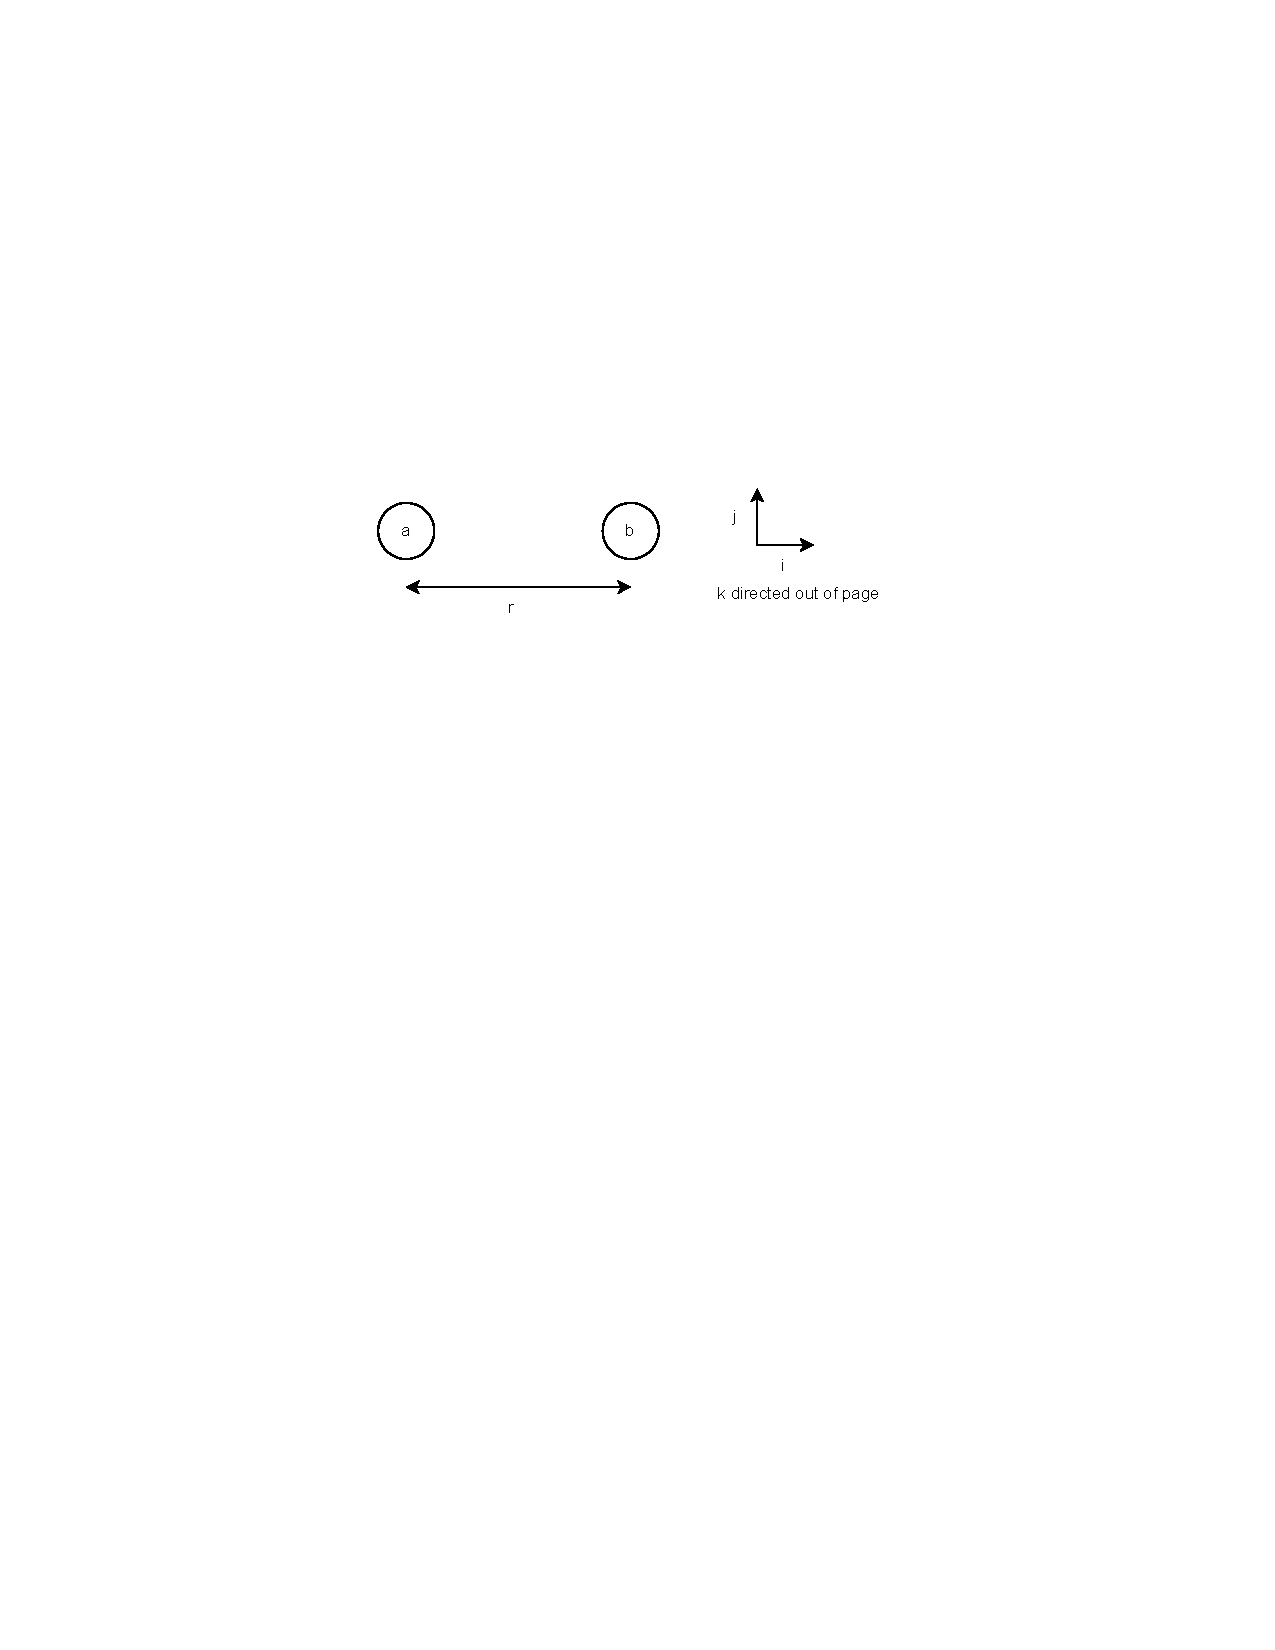
\includegraphics[width=0.6\textwidth]{two-charges-at-rest-cropped.pdf}
	\caption{Two point charges at rest}
	\label{fig:two-charges-at-rest}
\end{figure}


Scenario 2: The same as scenario 1, but both charges are moving with
constant velocity $v$ in the upwards direction (see
Figure~\ref{fig:two-charges-moving}).  Since they are moving they
create magnetic fields.

\begin{figure}[ht]
	\centering
	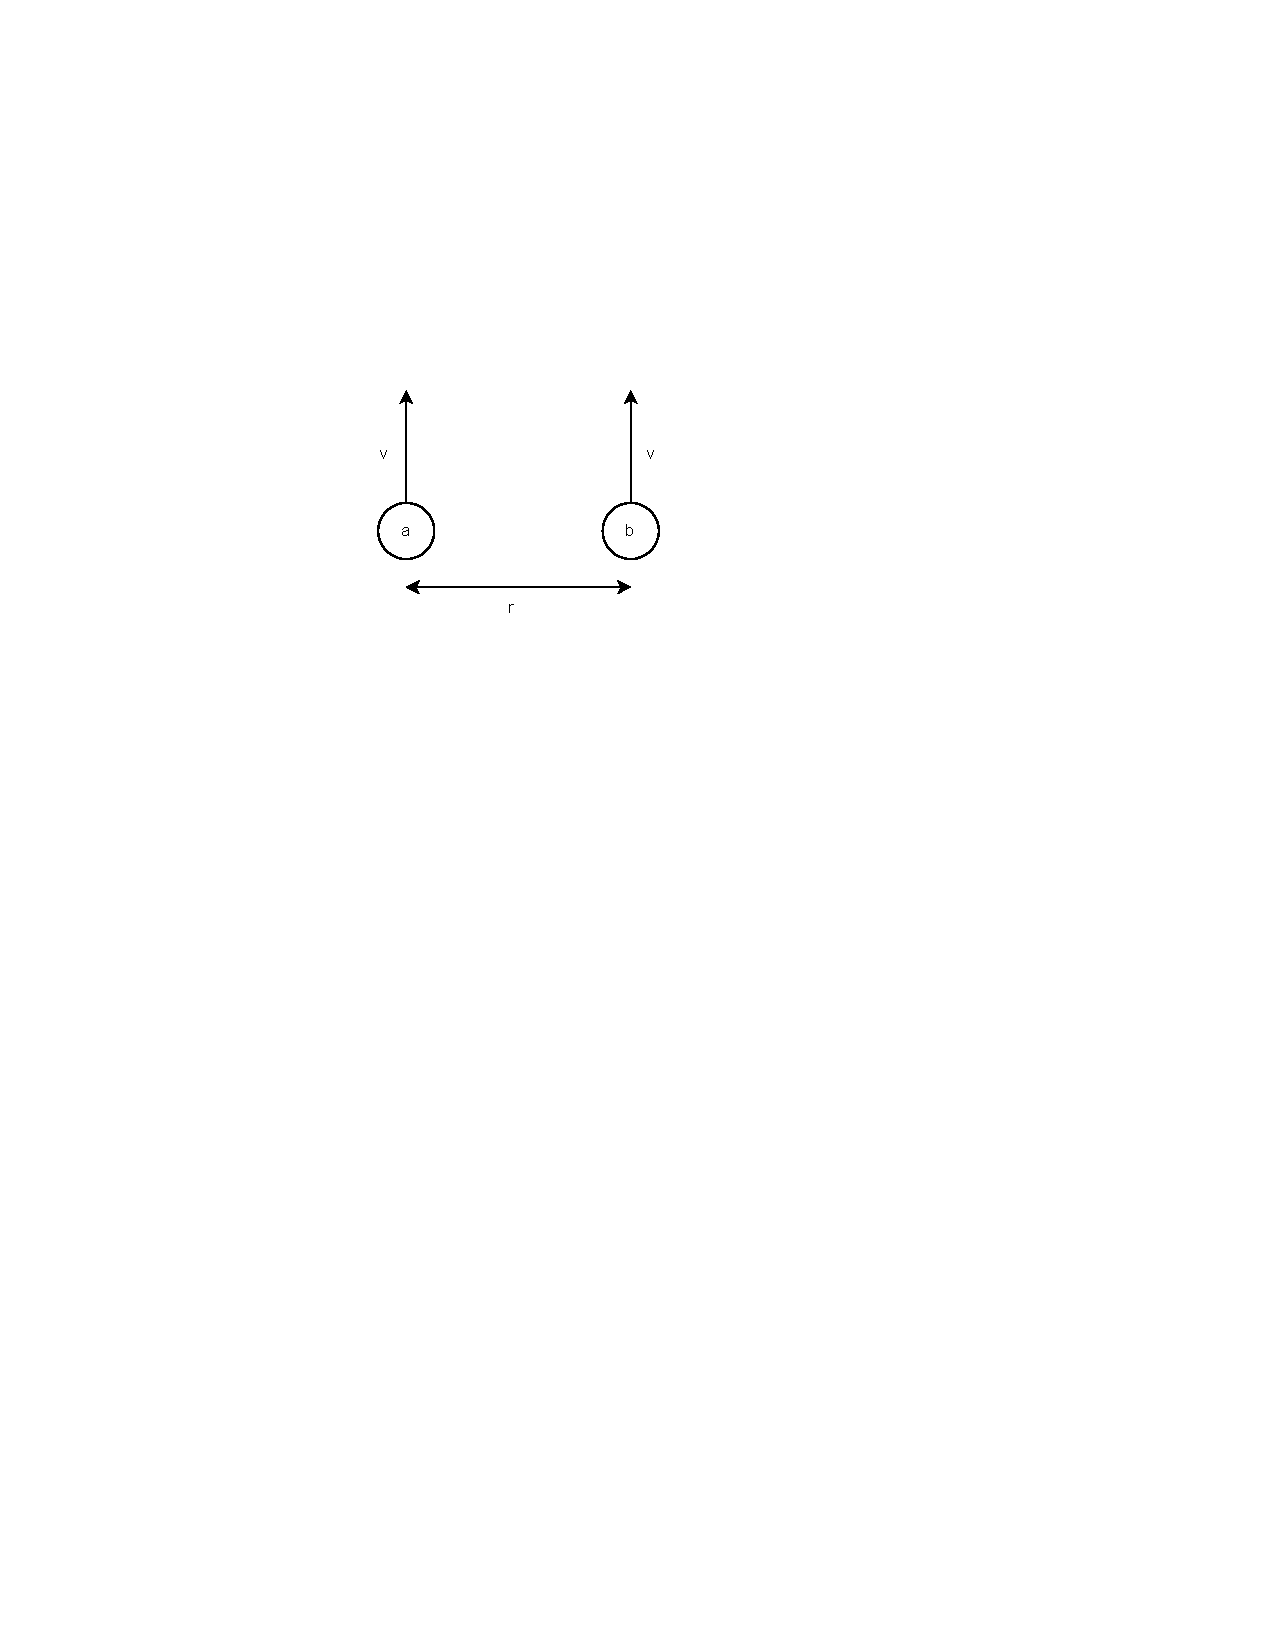
\includegraphics[width=0.4\textwidth]{two-charges-moving-cropped.pdf}
	\caption{Two point charges moving at same constant velocity}
	\label{fig:two-charges-moving}
\end{figure}

Questions:
\begin{itemize}
  \item What is the net force on charge $b$ in each scenario?
  \item Is it the same in both scenarios, or different?
  \item Why?
\end{itemize}


\subsection{Scenario 1: Both charges at rest}

As mentioned before, there is no current or motion of any charges in
this scenario, so no magnetic fields.  The electric repulsion force on
charge $b$ is easily calculated from Coulomb's Law~\cite{CoulombsLaw}.
Charge $b$ is to the right of charge $a$, so the direction of the force is
$\ihat$, away from charge $a$.

\begin{equation}
\vect{E}_1 = \frac{1}{4 \pi \epsilon_0} \frac{q}{r^2} \ihat \label{eq:E1}
\end{equation}

\begin{equation}
\vect{B}_1 = 0
\end{equation}

\begin{equation}
\vect{F}_1 = q(\vect{E}_1 + \vect{v} \times \vect{B}_1)
           = q \vect{E}_1   \label{eq:F1}
\end{equation}


\subsection{Scenario 2: Both charges with equal and constant velocity upwards}

\subsubsection{Scenario 2 calculated by electromagnetic field equations from Griffiths}

The Wikipedia page on the Biot-Savart
Law~\cite{EMFieldFromPointCharge} has a subsection titled ``Point
charge at constant velocity'' that says:

\begin{quote}
the Biot–Savart law applies only to steady currents and a point charge
moving in space does not constitute a steady current
\end{quote}

I will thus use the equations in that section to calculate the
electric and magnetic fields here.  The relevant parts of the
Wikipedia page are copied below.

\begin{quote}
In the case of a point charged particle $q$ moving at a constant
veclocity $\vect{v}$, Maxwell's equations give the following
expression for the electric field and magnetic field:
\end{quote}
\begin{align}
\vect{E} & = \frac{q}{4 \pi \epsilon_0} \frac{1-\beta^2}{(1-\beta^2 \sin^2 \theta)^{3/2}} \frac{{\rhat}'}{|r'|^2} \label{eq:EforPtChg} \\
\vect{B} & = \frac{1}{c^2} \vect{v} \times \vect{E} \label{eq:BforPtChg}
\end{align}
where:
\begin{itemize}
    \item ${\rhat}'$ is the unit vector pointing from the current
      (non-retarded) position of the particle to the point at which
      the field is being measured,
    \item $\beta = v/c$ is the speed in units of $c$, and
    \item $\theta$ is the angle between $\vect{v}$ and ${\rhat}'$.
\end{itemize}

The equations above appear to be identical to equations (10.75) and
(10.76) in Griffiths~\cite{Griffiths1998}.  Griffiths comments on the formula for the electric field:

\begin{quote}
Notice that $\vect{E}$ points along the line from the {\em present}
position of the particle.  This is an extraordinary coincidence, since
the ``message'' came from the retarded position.  Because of the
$\sin^2 \theta$ in the denominator, the field of a fast-moving charge
is flattened out like a pancake in the direction perpendicular to the
motion (Fig. 10.10).  In the forward and backward directions
$\vect{E}$ is reduced by a factor $(1 - v^2/c^2)$ relative to the
field of a charge at rest; in the perpendicular direction it is
{\em enhanced} by a factor $1 / \sqrt{ 1 - v^2/c^2}$.
\end{quote}

Calculation: To get the force on charge $b$, we first calculate the
$\vect{E}$ and $\vect{B}$ fields at the position of charge $b$.

Charge $b$ is directly to the right of charge $a$, so ${\rhat}' = \ihat$
and $\theta = 90^{\circ}$.

\begin{align}
\vect{E}_2
  & = \frac{q}{4 \pi \epsilon_0} \frac{1-\beta^2}{(1-\beta^2 \sin^2 \theta)^{3/2}} \frac{{\rhat}'}{|r'|^2} & & \text{${\rhat}' = \ihat$, $|r'| = r$, $\theta=90^{\circ}$, simplify fraction} \nonumber \\
  & = \frac{q}{4 \pi \epsilon_0} \frac{1}{(1-\beta^2)^{1/2}} \frac{\ihat}{r^2} & & \text{part of this is $\gamma$, by~\eqref{eq:E1} the rest is $\vect{E}_1$} \nonumber \\
  & = \gamma \vect{E}_1 \label{eq:E2value}
\end{align}

Note that $\vect{E}_2$ being $\gamma$ times larger than $\vect{E}_1$
is consistent with the comment from Griffiths above: ``in the
perpendicular direction it ($\vect{E}$) is {\em enhanced} by a factor
$1 / \sqrt{ 1 - v^2/c^2}$''.

\begin{align*}
\vect{F}_2
  & = q (\vect{E}_2 + \vect{v} \times \vect{B}_2)   & & \text{replace $\vect{B}_2$ with \eqref{eq:BforPtChg}} \\
  & = q (\vect{E}_2 + \vect{v} \times (\frac{1}{c^2} \vect{v} \times \vect{E}_2))  & & \vect{v} \times \vect{E}_2 = - v E_2 \khat \\
  & = q (\vect{E}_2 - \frac{v E_2}{c^2} \vect{v} \times \khat)  & & \vect{v} \times \khat = v \ihat \\
  & = q (\vect{E}_2 - \frac{v^2 E_2}{c^2} \ihat) \\
  & = q (1 - \frac{v^2}{c^2}) \vect{E}_2 \\
  & = \frac{q \vect{E}_2}{\gamma^2} & & \text{by~\eqref{eq:E2value} \ } \vect{E}_2 = \gamma \vect{E}_1 \\
  & = \frac{q \vect{E}_1}{\gamma} & & \text{by~\eqref{eq:F1} \ } \vect{F}_1 = q \vect{E}_1 \\
  & = \frac{\vect{F}_1}{\gamma}
\end{align*}

Thus $\vect{F}_2$ differs from $\vect{F}_1$ by a factor of $\gamma$.

TODO: Why?

I do not know how to check the answer below, but it appears that three
of the answers to an on-line question similar to
mine~\cite{PhysicsSEIsLorentzForceFrameIndependent} say that the
Lorentz force formula $\vect{F} = q(\vect{E} + \vect{v} \times
\vect{B})$ is {\em not} invariant in all inertial frames, but perhaps
a slightly modified version of that formula is invariant between
different inertial frames.  I quote one such answer below:

\begin{quote}
Just for completeness if permitted: Following Section 3.1 from the
book ``Gravitation'' of Misner, Thorne, and Wheeler the truly (at all
speeds) frame independent force is $\frac{dP}{d \tau} = \gamma (E + v
\times B)$ (in fact this is only the spacial component of the four
force).  $\tau$ is proper time and $\gamma$ the well-known Lorentz
Factor. -- Kurt G. Aug 28, 2021
\end{quote}


\subsubsection{Scenario 2 calculated by Heaviside-Feynman formula}

The Wikipedia page on Jefimenko's Equations~\cite{JefimenkosEquations}
has a subsection titled ``Heaviside-Feynman formula'' that gives
equations for the electric and magnetic field at a point due to a
single moving point charge.

\begin{align}
\vect{E} & = \frac{-q}{4 \pi \epsilon_0}
             \left[
               \frac{\vect{e}_{r'}}{r'^2}
               + \frac{r'}{c} \frac{d}{dt} \left( \frac{\vect{e}_{r'}}{r'^2} \right)
               + \frac{1}{c^2} \frac{d^2}{dt^2} \vect{e}_{r'}
             \right]
             \label{eq:HF-EforPtChg} \\
\vect{B} & = - \vect{e}_{r'} \times \frac{\vect{E}}{c}
             \label{eq:HF-BforPtChg}
\end{align}

Here $\vect{e}_{r'}$ is a unit vector pointing from the observer to
the charge and $r'$ is the distance between observer and charge.
Since the electromagnetic field propagates at the speed of light, both
of these quantities are evaluated at the retarted time $t - r'/c$.

I believe ``observer'' above means ``the position for which we are
calculating $E$ and $B$ fields''.

Assume here that the point charges are kept at distance $r$ apart from
each other, always horizontally, e.g. because they are connected by a
stiff insulating rod.  This simplifies our job of calculating $E$,
because then $\vect{e}_{r'}$ and $r'$ are unchanging over time, and
their derivates are thus 0.

We want to calculate $r'$ as the vector from the position of charge
$b$ to the position where charge $a$ was when it emitted an electric
field propagated at speed $c$ to $b$.  See
Figure~\ref{fig:retarded-position}.

\begin{figure}[ht]
	\centering
	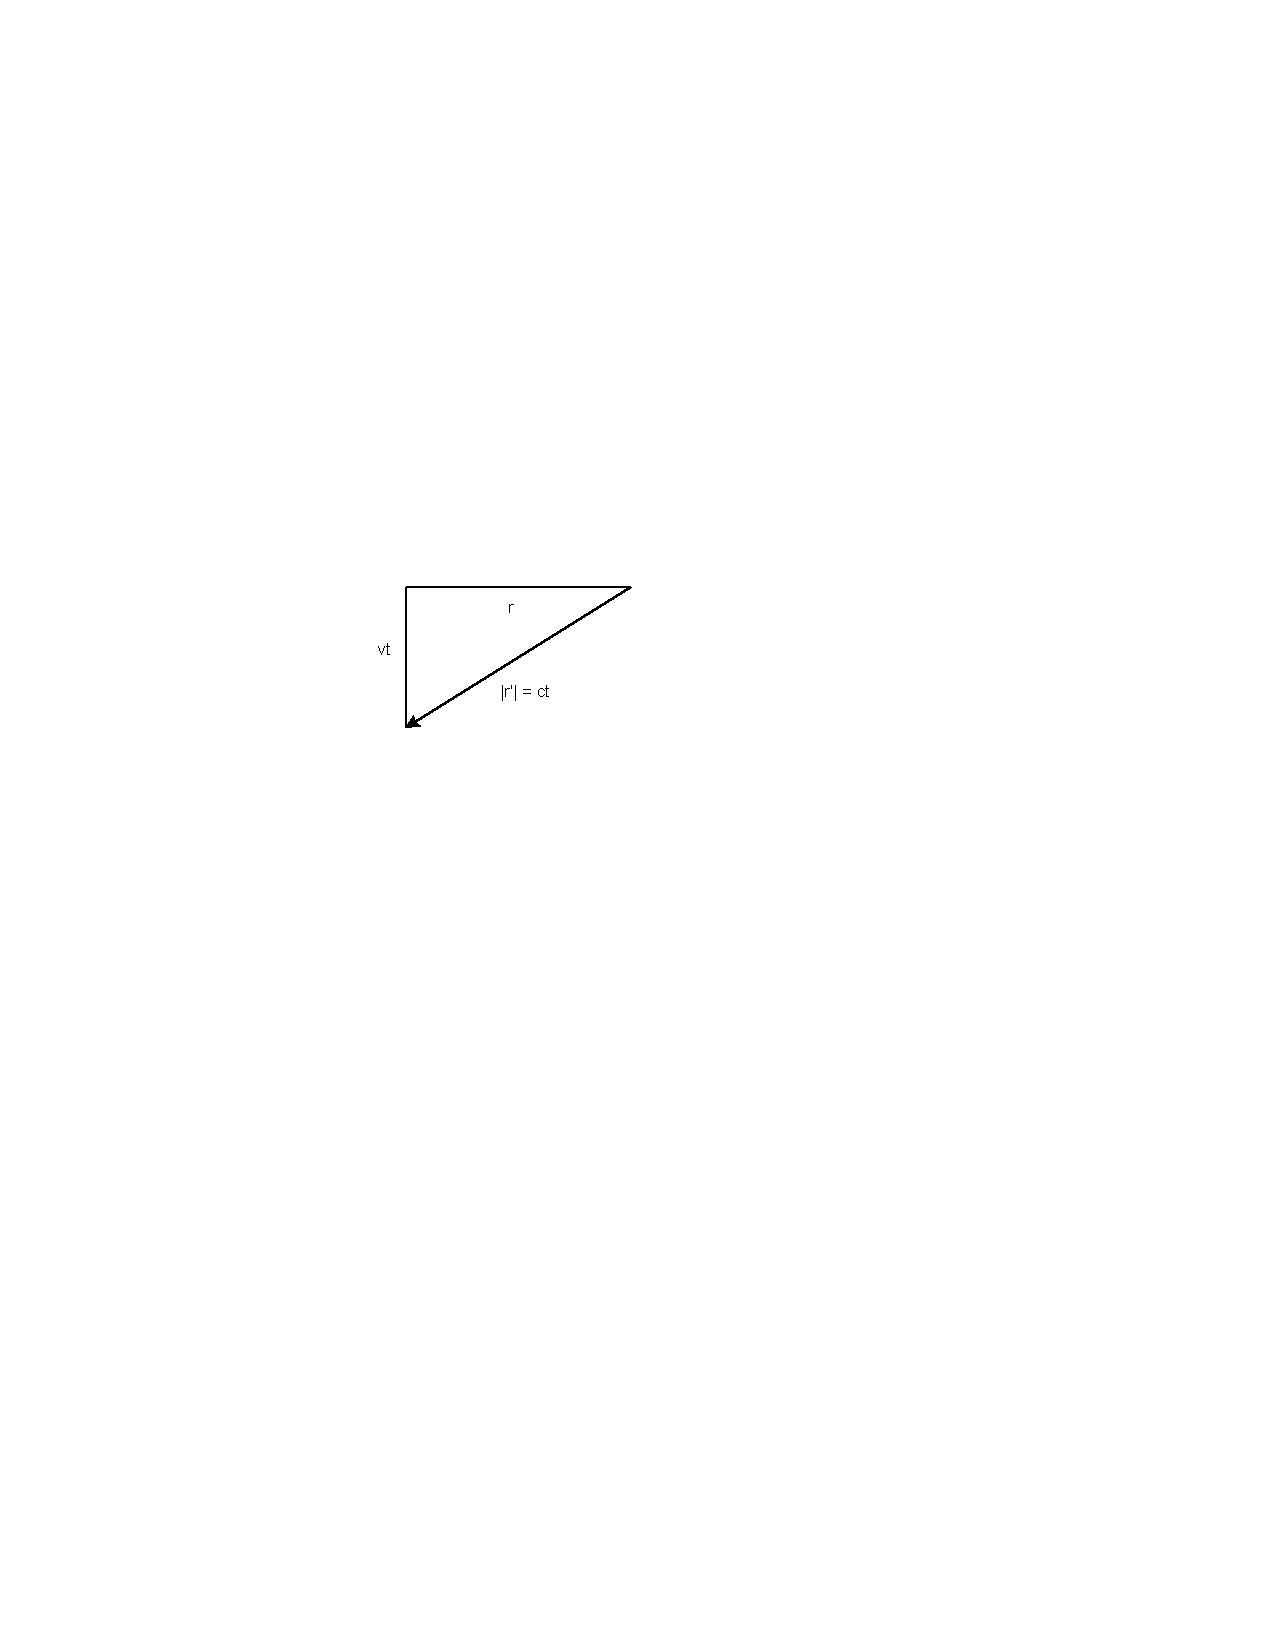
\includegraphics[width=0.5\textwidth]{retarded-position-cropped.pdf}
	\caption{The retarded position of charge $a$ from charge $b$}
	\label{fig:retarded-position}
\end{figure}

Solve for $t$ using Pythagorean theorem since $r$ and $v$ are known
constants:
\begin{align*}
r^2 + (vt)^2 & = (ct)^2 \\
t^2 (c^2 - v^2) & = r^2 \\
t^2 & = \frac{r^2}{c^2 - v^2} \\
t & = \frac{r}{\sqrt{c^2-v^2}} \\
  & = \frac{r}{c \sqrt{1 - v^2/c^2}} \\
  & = \gamma r / c
\end{align*}

This gives us $r' = ct = \gamma r$, and $\vect{e}_{r'}$ is:

\begin{align*}
\vect{e}_{r'} & = \frac{-r \ihat - (\gamma r v / c) \jhat}{\gamma r} \\
  & = - \frac{1}{\gamma} \ihat - \frac{v}{c} \jhat
\end{align*}

Plugging in this value for $\vect{e}_{r'}$ into
Equation~\eqref{eq:HF-EforPtChg} gives:

\begin{align*}
\vect{E}_3 & = \frac{q}{4 \pi \epsilon_0}
             \left[
               \frac{\frac{1}{\gamma} \ihat + \frac{v}{c} \jhat}{\gamma^2 r^2}
             \right]
\end{align*}

Note that $\vect{E}_3$ is parallel to $\vect{e}_{r'}$, thus
$\vect{B}_3$ from Equation~\eqref{eq:HF-BforPtChg} is 0.

This gives the force on charge $b$ as:
\begin{align*}
\vect{F}_3
  & = q (\vect{E}_3 + \vect{v} \times \vect{B}_3) \\
  & = q \vect{E}_3
\end{align*}
The direction of $\vect{F}_3$ is different than $\vect{F}_1$ and $\vect{F}_2$.
Below is the relative magnitude of $\vect{E}_3$ to $\vect{E}_1$:
\begin{align*}
E_3 & = \frac{1}{\gamma^2} E_1 \\
F_3 & = \frac{1}{\gamma^2} F_1
\end{align*}

TODO: It seems {\em very} odd to me that $\vect{B}_3 = 0$.

After Feynman explains what the retarded direction and distance
$\vect{r'}$ is, he says~\cite{FeynmanLecturesVolICh28}:
\begin{quote}
That would be easy enough to understand, too, but it is also
wrong.  The whole thing is much more complicated.
\end{quote}
Unfortunately there are no footnotes or citation to explain what he
meant by this.


\section{Simple time scenarios in special relativity and Lorentz Ether Theory}
\label{sec:simple-sr-time}

Definitions of some terms:
\begin{align}
  \beta & = v / c \label{defn:betaB} & & \text{the {\em relativistic velocity}, or {\em velocity ratio}} \\
  \gamma & = \frac{1}{\sqrt{1 - \beta^2}} & & \text{the {\em Lorentz factor}} \label{defn:LorentzFactor} \\
  D & = \sqrt{ \frac{1 + \beta}{1 - \beta} } & & \text{the {\em Doppler factor}} \label{defn:DopplerFactor}
\end{align}
Later in this article we typically write a subscript after $v$,
$\beta$, $\gamma$, and $D$ to indicate the entity that has the
relevant velocity $v$.  The context should make it clear in what
inertial frame that velocity $v$ applies.

We will use these definitions in scenarios where $-c < v < c$.
Thus:
\begin{align}
-1 & \leq \beta < 1 \nonumber \\
\gamma & \geq 1 & & \text{$\gamma$ increases as $|\beta|$ does} \nonumber \\
\lim_{\beta \rightarrow 1} \gamma & = +\infty \nonumber \\
\lim_{\beta \rightarrow -1} \gamma & = +\infty \nonumber \\
D & = \gamma (1+\beta) > 0 & & \text{$D$ increases as $\beta$ does} \label{eqn:DaltFormula}
\end{align}


\subsection{Special Relativity Scenario 1a: Two entities moving relative to each other at constant velocity}
\label{sec:scen1a}

$A$ is at rest.  $B$ is moving at constant velocity $v_B$ relative to $A$,
either directly away from $A$, or directly towards $A$.
$v_B > 0$ means $B$ moves away from $A$.
$v_B < 0$ means $B$ moves towards $A$.


\subsubsection{$B$ sends periodic pulses to $A$}
\label{sec:scen1a-BtoA}

$B$ uses his local clock to time the sending of light pulses to $A$,
sending pulses once every time interval $T$.
At what period does $A$ receive the pulses?

Define $q_A(n)$ to be the time on A's clock when the $n$-th pulse is
transmitted by $B$, and $q_B(n)$ to be the time on B's clock when it
transmits the $n$-th pulse.

$q_B(n) = nT$ by the setup of the experiment.

By the assumptions of special relativity, $A$ deduces that $B$'s clock
is running $\gamma_B$ times slower than $A$'s clock.  Note: $A$ cannot
directly observe $B$'s clock, as it is too far away.  From this $A$
also deduces:
\begin{equation}
q_A(n) = \gamma_B nT + \Delta  \label{eqn:scen1a-timeA}
\end{equation}
$\Delta$ is the time that $A$ reads on his clock
when $B$ reads 0 on his clock.  The value of $\Delta$
is irrelevant to the final result we seek.

$B$'s distance from $A$ at $A$'s time $t_A$ is
$x_B(t_A) = I_B + v_B t_A$.
$I_B > 0$ is $B$'s initial distance from $A$ at $t_A=0$.
The value of $I_B$ is also irrelevant to the final result we seek,
as long as it is large enough that $x_B(t_A) > 0$ remains
true while $B$ emits all of the pulses we consider (two pulses is enough).

Also by the assumptions of special relativity, $A$ deduces that $B$'s
pulse signal will propagate at the one-way speed $c$.  The pulse will
thus take time $x_B(q_A(n))/c$ to propagate to $A$.

$A$'s clock thus shows time $r_A(n) = q_A(n) + x_B(q_A(n))/c$ when the $n$-th
pulse arrives at $A$.  With a little algebra:
\begin{align*}
r_A(n)
  & = q_A(n) + x_B(q_A(n))/c & & \text{definition of $r_A(n)$} \\
  & = q_A(n) + (I_B + v_B q_A(n))/c & & \text{substitute equation for $x_B$} \\
  & = (1 + v_B/c) q_A(n) + I_B/c & & \text{rearrangement by algebra} \\
  & = (1 + \beta_B) (\gamma_B nT + \Delta) + I_B/c & & \text{Defn.~\eqref{defn:betaB} and Eqn.~\eqref{eqn:scen1a-timeA}} \\
  & = (1 + \beta_B) \gamma_B Tn + ((1 + \beta_B) \Delta + I_B/c) & & \text{algebra to collect all terms independent of $n$ at the end}
\end{align*}
The time that $A$ measures on his clock between two consecutive received
pulses is:
\begin{align*}
r_A(n+1) - r_A(n)
  & = (1 + \beta_B) \gamma_B T & & \text{by calculation of $r_A(n)$ above} \\
  & = D_B T & & \text{Eqn.~\eqref{eqn:DaltFormula}}
\end{align*}
The pulses arrive at $A$ with a period of $D_B T$ measured on $A$'s clock.

Suppose that $A$ knows somehow the period $T$ that $B$ uses as its
period for transmitting pulses, e.g. because they agreed and arranged
this beforehand.  Then $A$ can measure the period between received
pulses on his clock and divide it by $T$ to calculate $D_B$.
By Corollary~\ref{cor:DdeterminesBeta} in
Appendix~\ref{app:DopplerFactor}, $A$ can calculate from $D_B$ the one
value of $\beta_B$ in the range $(-1, 1)$ that corresponds to it, and
$v_B$ in the range $(-c, +c)$.

Note 1: There is {\em nothing} in this derivation that relies upon prior
knowledge of the Doppler factor, or under what conditions it is
applicable.  That expression arose in
the process of calculating the answer, using only the assumptions that
light moves isotropically at speed $c$ in $A$'s frame, and that $A$
can deduce that $B$'s clock is running $\gamma_B$ times slower than
$A$'s clock.


\subsubsection{$A$ sends periodic pulses to $B$}
\label{sec:scen1a-AtoB}

Now $A$ uses his local clock to time the sending of light pulses to $B$,
sending pulses once every time interval $T$.
At what period does $B$ receive the pulses?

While we could switch perspectives to $B$'s inertial frame, we will
not.  Instead, we are going to do all of the calculations in $A$'s
inertial frame.

The definitions of Section~\ref{sec:simple-sr-time} remain the same here, but note
that the values of $q_A(n)$ and $q_B(n)$ here are {\em different} than
those in Section~\ref{sec:scen1a-BtoA}.

Define $q_A(n) = nT$ to be the time on A's clock when it transmits its
$n$-th pulse.

At all times $t_A$, $B$ is a distance $x_B(t_A) = I_B + v_B t_A$ away from $A$.
As in the previous section, $I_B > 0$ is any value large enough
that $x_B(t_A)$ remains positive while $A$ emits all of the pulses we consider.

$A$ assumes by special relativity that its pulse propagates with one-way
speed $c$ to $B$.  The pulse's position at time $t_A \geq q_A(n)$ is
$c(t_A - q_A(n))$.

On $A$'s clock, $A$ deduces that
its $n$-th pulse catches up to $B$ at a time $r_A(n)$ that satisfies the equation:
\begin{align}
x_B(r_A(n)) & = c(r_A(n) - q_A(n)) & & \text{$B$'s position equals light pulse's position} \nonumber \\
I_B + v_B r_A(n) & = c(r_A(n) - nT) & & \text{substitute for defns. of $x_B$ and $q_A(n)$} \\
I_B/c + (v_B/c) r_A(n) & = r_A(n) - nT & & \text{divide by $c$} \nonumber \\
nT + I_B/c & = (1 - v_B/c) r_A(n) & & \text{a little more algebra} \nonumber \\
r_A(n) & = \frac{nT}{1 - v_B/c} + \frac{I_B}{c-v_B} & & \text{divide by $(1-v_B/c)$} \nonumber \\
r_A(n) & = \frac{nT}{1 - \beta_B} + \frac{I_B}{c-v_B} & & \text{Defn.\eqref{defn:betaB}} \label{eqn:scen1a-Arecvtime}
\end{align}
By the assumptions of special relativity, $A$ deduces that $B$'s clock
is running $\gamma_B$ times slower than $A$'s clock.
Thus $B$'s time when receiving the $n$-th pulse is
the following, where $\Delta$ is the time that $B$ reads on his clock
when $A$ reads 0 on his clock (as in the previous section,
the value of $\Delta$ is irrelevant in our final answer):
\begin{align*}
r_B(n) & = r_A(n) / \gamma_B + \Delta & & \text{$B$'s clock slower by factor $\gamma_B$} \\
       & = \frac{nT}{\gamma_B(1 - \beta_B)} + (\frac{I_B}{\gamma_B(c-v_B)} + \Delta) & & \text{Eqn.~\eqref{eqn:scen1a-Arecvtime}, move things independent of $n$ to end}
\end{align*}
The time that $B$ measures on his clock between two consecutive received
pulses is:
\begin{align*}
r_B(n+1) - r_B(n)
  & = \frac{T}{\gamma_B(1 - \beta_B)} & & \text{by calculation of $r_B(n)$ above} \\
  & = \frac{\sqrt{1 - \beta_B^2}}{1 - \beta_B} T & & \text{Defn.~\eqref{defn:LorentzFactor}} \\
  & = \sqrt{ \frac{1 + \beta_B}{1 - \beta_B} } T & & \text{a little algebra} \\
  & = D_B T & & \text{Defn.~\eqref{defn:DopplerFactor}}
\end{align*}
$B$ will observe pulses arriving with period $D_B T$ according to
$B$'s clock.

While this formula for the period between received pulses
is very similar to the one in the previous section, note that
both the sending and receiving period are being measured on different
clocks than there.

As in the previous section, if $B$ somehow knows $T$,
he can measure the interal between receive pulses,
divide it by $T$ to calculate $D_B$,
then use that to calculate $\beta_B$ and $v_B$.


\subsubsection{Relationship to Lorentz Ether Theory}
\label{sec:scen1a-LET}

Note in Sections~\ref{sec:scen1a-BtoA} and~\ref{sec:scen1a-AtoB}, that
except for algebra and the definitions of symbols from
Section~\ref{sec:simple-sr-time}, the only assumptions we used from special relativity were:
\begin{itemize}
\item The one-way speed of light is $c$ in all directions in $A$'s
  inertial frame.
\item In $A$'s frame, $B$'s clock runs at a slower rate, by a factor
  of $1/\gamma_B$, relative to $A$'s clock.
\end{itemize}
By Lorentz Ether Theory, suppose that somehow we know that $A$ is at
rest relative to the ether, then:
\begin{itemize}
\item The one-way speed of light is $c$ in all directions relative to
  the ether, and thus also relative to $A$.
\item $B$ is moving at velocity $v_B$ relative to the ether, and thus
  $B$'s clock physically runs at a slower rate, $1/\gamma_B$ times as
  fast as the true time.  $A$'s clock runs at the full rate of true
  time, the same as any other clocks at rest relative to the ether.
\end{itemize}

TODO: Find a way to explain the following better.

I had heard from a not-yet-in-depth learning about special relativity
that when $A$ and $B$ are moving at constant velocity towards or away
from each other, that $A$ observed that $B$'s clock ran slower by a
factor of $\gamma$, and $B$ observed that $A$'s clock ran slower by a
factor of $\gamma$.  (Note: I do not claim that those are fully
precise statements, but there is definitely a sense in which special
relativity does say something similar to this.)

In $A$'s frame observing $B$'s clock run slower, that seems perfectly
consistent with Lorentz Ether Theory's statement that if $A$ is at
rest relative to the ether, and $B$ moves at constant velocity $v_B$
relative to the ether, that $B$ experiences duration dilation,
i.e. its clock physically runs slower than $A$'s by a factor of
$\gamma_B$.  In this situation $A$'s clock runs at full speed,
i.e. $\gamma_B$ times {\em faster} than $B$'s.

But what about Lorentz Ether Theory's position on the converse
statement?  That is, from $B$'s point of view, does $B$ observe $A$'s
clock running $\gamma_B$ times slower?  If so, how can that possibly
make sense?

I now believe that the answer is that the statements in special
relativity can be made a bit more precise by saying something like
this: Because $A$ is following special relativity's assumptions,
i.e. in $A$'s frame the speed of light propagates isotropically at
constant speed $c$, therefore $A$ can deduce that any clocks moving at
constant speed $v$ directly towards or away from $A$ run $\gamma$
times slower, and make further calculations from that deduction.

$A$ does not actually {\em observe} such clocks directly over any
appreciable interval of time, so they are always, or almost always, so
far away that $A$ cannot make {\em any} direct observations of how
fast such clocks are running.  By ``direct'' observations I mean
``with light propagation delay very close to 0 between $A$ and the
entity being observed''.

Suppose in some future context of knowledge that not only is Lorentz
Ether Theory proven, but in such a way that we know how to measure our
speed relative to the ether.

Then, in the scanario described, we would know that $A$'s clock is
running at full speed, and light propagates isotropically at constant
speed $c$ relative to the ether, and thus also relative to $A$.

Everyone with this knowledge would be able to deduce that $B$'s clock
is running $\gamma$ times slower than full speed.  Also, that
$A$'s clock is running $\gamma$ times {\em faster} than $B$'s clock
(and that all of $A$'s local physical processes are proceeding
$\gamma$ times faster than similar local physical processes of $B$).

Further, light does {\em not} propagate at the same speed in all
directions relative to $B$.  It does so only with respect to the
ether.

We could also prove that if one chose to make calculations using
special relativity's assumptions in $B$'s frame, one would get the
same answers to these calculations that you do when using Lorentz
Ether Theory.

A hint of corroboration can be seen in the Wikipedia page on time
dilation, which says in the introduction~\cite{WikipediaTimeDilation}:
\begin{quote}
The dilation compares ``wristwatch'' clock readings between events
measured in different inertial frames and is not observed by visual
comparison of clocks across moving frames.
\end{quote}

It seems that any statement similar to:
\begin{itemize}
\item $A$ observes $B$'s clock running slower than their own.
\end{itemize}
could be said in much more detail as either of the following:
\begin{itemize}
\item In accordance with special relativity's time synchronization
  convention that light propagates in $A$'s inertial frame
  isotropically with speed $c$, $A$ deduces that $B$'s clock runs
  slower than $A$'s.
\item $A$ deduces, using the postulate that light moves isotropically
  at speed $c$, that $B$’s clock runs slower, and can then make
  further consistent calculations based on this deduction.
\end{itemize}
And you can swap $A$ and $B$ in that statement.  Without defining new
precise terminology, a shorter precise statement would perhaps be:
\begin{itemize}
\item According to SR, in $A$'s inertial frame we deduce that $B$'s
  clock runs slower.
\end{itemize}


\subsection{Special Relativity Scenario 1b: Three entities, two of them moving at constant velocity}
\label{sec:scen1b}

$A$ is at rest.
$B$ is moving at constant velocity $v_B$ relative to $A$,
which is away from $A$ if $v_B > 0$, or towards $A$ if $v_B < 0$.
$C$ is moving at constant velocity $v_C$ relative to $A$,
with same sign conventions as $B$'s velocity.

For $B$ sending periodic pulses to $A$ or vice versa, everything in
Sections~\ref{sec:scen1a-BtoA} and~\ref{sec:scen1a-AtoB} applies without
change.
For $C$ sending periodic pulses to $A$ or vice versa, everything in
Section~\ref{sec:scen1a-BtoA} and~\ref{sec:scen1a-AtoB} applies,
except replace $B$ subscripts
with $C$ subscripts, i.e. use $v_C$, $\gamma_C$, $\beta_C$, and $D_C$.

So it is only pulses between $B$ and $C$ that might present something
new here.

Our calculations in the following sections for pulse signals between
$B$ and $C$ assume that throughout the entire duration of sending and
receiving the pulses of interest, either:
\begin{itemize}
\item $B$'s position according to its $x$ coordinate is always less
  than $C$'s $x$ coordinate, or
\item $B$'s position according to its $x$ coordinate is always greater
  than $C$'s $x$ coordinate, or
\end{itemize}
If that condition is ever violated because $B$ crosses paths with $C$,
the results presented here are no longer applicable after that occurs.
We use $I_B$ and $I_C$ to represent their initial distances from $A$,
and require that these positions, combined with their velocities, will
ensure this.


\subsubsection{$B$ sends periodic pulses to $C$}
\label{sec:scen1b-BtoCLETfriendly}

$B$ uses his local clock to time the sending of light pulses to $C$,
sending pulses once every time interval $T$, according to $B$'s clock.
At what period does $C$ receive the pulses?

To make the calculations as easily applicable to Lorentz Ether Theory
as possible, all calculations will be done in $A$'s inertial frame.

Define $q_A(n)$ and $q_B(n)$ the same way as they were in
Section~\ref{sec:scen1a-BtoA}.  As explained there, when $A$ makes the
assumptions according to special relativity theory:
\begin{align}
q_B(n) & = nT & & \text{by the setup of the experiment} \nonumber \\
t_A & = \gamma_B t_B + \Delta_B & & \text{$B$'s clock runs $\gamma_B$ times slower than $A$'s} \nonumber \\
q_A(n) & = \gamma_B nT + \Delta_B \label{eqn:scen1b-timeArelB} \\
t_A & = \gamma_C t_C + \Delta_C & & \text{$C$'s clock runs $\gamma_C$ times slower than $A$'s} \nonumber \\
t_C & = t_A/\gamma_C - \Delta_C/\gamma_C & & \text{equivalent to previous equation, but solved for $t_C$} \label{eqn:scen1b-timeArelC} \\
x_B(t_A) & = I_B + v_B t_A & & \text{relationship of $B$'s position and time, in $A$'s frame} \label{eqn:scen1b-posB} \\
x_C(t_A) & = I_C + v_C t_A & & \text{relationship of $C$'s position and time, in $A$'s frame} \label{eqn:scen1b-posC}
\end{align}
Also by special relativity assumptions, $A$ considers the pulse to
travel from $B$ to $C$ at constant speed $c$.
The $n$-th pulse is emitted at time $q_A(n)$ in $A$'s frame,
so its position as a function of $A$'s time $t_A$ is given by
$l_A(n, t_A)$ below.
Note that $d$ is 1 if $C$'s $x$ coordinate is greater than $B$'s, and
thus the pulse of interest is moving in the increasing $x$
direction.  Otherwise $d$ is -1.
\begin{align*}
l_A(n, t_A)
  & = \text{position of $B$ when emitted} \\
  &   + \text{distance traveled after emission} \\
  & = x_B(q_A(n)) + d (t_A - q_A(n)) c & & \text{for any time $t_A \geq q_A(n)$} \\
  & = I_B + v_B q_A(n) + d (t_A - q_A(n)) c & & \text{substitute Eqn.~\eqref{eqn:scen1b-posB}} \\
  & = (v_B - dc) q_A(n) + dc t_A + I_B & & \text{algebra} \\
  & = (v_B - dc) \gamma_B nT + dc t_A + ((v_B-c)\Delta_B + I_B) & & \text{substitute Eqn.~\eqref{eqn:scen1b-timeArelB}} \\
  & = (v_B - dc) \gamma_B nT + dc t_A + Z & & \text{$Z$ is constants, independent of $n$ and $t_A$}
\end{align*}
To find $A$'s time $r_A(n)$ when $C$ receives the pulse,
solve for the time that makes the pulse position the same as $C$'s position:
\begin{align*}
x_C(r_A(n)) & = l_A(n, r_A(n)) \\
I_C + v_C r_A(n) & = (v_B - dc) \gamma_B nT + dc r_A(n) + Z & & \text{substitute Eqn.~\eqref{eqn:scen1b-posC}} \\
(v_C - dc) r_A(n) & = (v_B - dc) \gamma_B nT + (Z - I_C) & & \text{algebra} \\
r_A(n) & = \frac{v_B - dc}{v_C - dc} \gamma_B nT + \frac{Z - I_C}{v_C - c} & & \text{divide by $v_C-dc$} \\
r_A(n) & = \frac{d - \beta_B}{d -  \beta_C} \gamma_B nT + \frac{Z - I_C}{v_C - c} & & \text{defn. of $\beta_B, \beta_C$} \\
r_A(n) & = \frac{d - \beta_B}{d - \beta_C} \gamma_B nT + Y & & \text{$Y$ is a constant, independent of $n$}
\end{align*}
According to $A$ and its special relativity assumptions,
$C$'s clock runs slower, at a rate $1/\gamma_C$ times that of $A$'s clock.
So $C$'s time $r_C(n)$ to receive the $n$-th pulse sent by $B$ is:
\begin{align*}
r_C(n) & = \frac{1}{\gamma_C} r_A(n) - \Delta_C/\gamma_C & & \text{Eqn.~\eqref{eqn:scen1b-timeArelC}} \\
       & = \frac{\gamma_B}{\gamma_C} \left( \frac{d-\beta_B}{d-\beta_C} \right) nT + \frac{Y-\Delta_C}{\gamma_C}
\end{align*}
The time that $B$ measures on his clock between two consecutive received
pulses is:
\begin{align*}
r_C(n+1) - r_C(n)
  & = \frac{\gamma_B}{\gamma_C} \left( \frac{d-\beta_B}{d-\beta_C} \right) T \\
  & = \sqrt{ \frac{1-\beta_C^2}{1-\beta_B^2} } \left( \frac{d-\beta_B}{d-\beta_C} \right) T & & \text{Defn.~\eqref{defn:LorentzFactor}}
\end{align*}
From here there are two slightly different cases, depending on the
value of $d$.  First let us finish the problem for the case of $d=1$,
when $C$ is at a greater $x$ coordinate than $B$:
\begin{align*}
r_C(n+1) - r_C(n)
  & = \sqrt{ \frac{1+\beta_C}{1-\beta_C} } \sqrt { \frac{1-\beta_B}{1+\beta_B} } T & & \text{algebra} \\
  & = ( D_C / D_B ) T & & \text{defn. of $D_B, D_C$}
\end{align*}
Now for the case $d=-1$, when $C$ is at a lesser $x$ coordinate than
$B$:
\begin{align*}
r_C(n+1) - r_C(n)
  & = \sqrt{ \frac{1-\beta_C^2}{1-\beta_B^2} } \left( \frac{-1-\beta_B}{-1-\beta_C} \right) T \\
  & = \sqrt{ \frac{1-\beta_C^2}{1-\beta_B^2} } \left( \frac{1+\beta_B}{1+\beta_C} \right) T & & \text{algebra} \\
  & = \sqrt{ \frac{1-\beta_C}{1+\beta_C} } \sqrt { \frac{1+\beta_B}{1-\beta_B} } T & & \text{algebra} \\
  & = ( D_B / D_C ) T & & \text{defn. of $D_B, D_C$}
\end{align*}

So when $B$ sends pulses with period $T$ according to $B$'s clock, and
$C$ is at a greater $x$ coordinate than $B$, $C$ receives from $B$
pulses with period $(D_C / D_B) T$ on $C$'s clock.  If $C$ is at a
lesser $x$ coordinate than $B$, $C$ receives pulses with period
$(D_B / D_C) T$ on $C$'s clock.

Since $D > 0$ and it increases with $\beta$ (see
Appendix~\ref{app:DopplerFactor}), and thus also with $v$,
$(D_C / D_B)$ is greater than 1 if $v_C > v_B$, otherwise less than 1,
and $(D_B / D_C)$ is greater than 1 if $v_C < v_B$.

\begin{tabularx}{1.0\textwidth}{|p{4cm}|p{4cm}|p{4cm}|}
\cline{1-3} \\
       & $v_c < v_B$ & $v_c > v_B$ \\ \cline{1-3}
$C$ is at greater $x$ coordinate than $B$ & $C$ and $B$ getting closer.  $(D_C / D_B) < 1$ & $C$ and $B$ getting further.  $(D_C / D_B) > 1$ \\ \cline{1-3}
$C$ is at lesser $x$ coordinate than $B$ & $C$ and $B$ getting further.  $(D_B / D_C) > 1$ & $C$ and $B$ getting closer.  $(D_B / D_C) < 1$ \\ \cline{1-3}
\end{tabularx}

All of these cases are a bit annoying.  It is good to note that as
long as you use the one of $D_C / D_B$ and $D_B / D_C$ that is greater
than 1 if $B$ and $C$ are moving away relative to each other, and the
one that is less than 1 if $B$ and $C$ are getting closer over time,
you will get the right answer.

Aside: If you are curious, the answer provided by ChatGPT for solving
this problem can be found in Appendix~\ref{sec:scen1b-BtoCdoublecheck}.

Near the end of Sections~\ref{sec:scen1a-BtoA} and~\ref{sec:scen1a-AtoB},
we noted that if the receiver knew somehow the period $T$ that the
sender is sending pulses, the receiver could calculate a $D$ value
that enabled the receiver to determine what the velocity of $B$ is.

In the current scenario, the receiver $C$, if it knows $T$, can
measure the time interval between pulses it receives, divide by $T$,
and calculate $(D_C / D_B)$.

Thus, with the measurement of the interval between received pulses,
given any two of $T$, $v_A$, and $v_B$, $C$ can calculate the other
one of those (and given values for two of those quantities, there is
only one value possible for the remaining one).
But from the measurement of the interval between received pulses and
$T$, that is not enough information for $C$ to calculate either one of
$v_B$ or $v_C$.

However, it {\em can} do the following.  Define $D_r = (D_C / D_B)$.
From Corollary~\ref{thm:velSubLeadsToDopplerFQuotient} in
Appendix~\ref{app:DopplerFactor}, we know that if
$\beta_r = \beta_C \ominus \beta_B$ for some $\beta_C, \beta_B$ values
in the range $(-1, +1)$, then $D_r = D_C / D_B$.

TODO: I am fairly certain it is straightforward to prove the converse:
If in this scenario $C$ calculates the value value of $D_r$, then
calculates $\beta_r = (D_r^2-1)/(D_r^2+1)$, then the only possible
pairs of values $\beta_C, \beta_B$ that could have given this
measurement are those satisfying $\beta_r = \beta_C \ominus \beta_B$.
There are an unlimited number of such pairs of values.

This strongly suggests that the receiver can calculate the
{\em relative} velocity between $B$ and $C$, at least in some sense.
I am not sure yet how to explain that further.

Also note that if we follow Lorentz Ether Theory, but we have no
knowledge of how to determine our motion relative to the ether, these
results show that the receiver can, with knowledge of the sender's
period $T$, still calculate this kind of relative velocity described,
which is interesting.


\subsubsection{$C$ sends periodic pulses to $B$}
\label{sec:scen1b-CtoBLETfriendly}

The derivation is nearly identical to that in
Section~\ref{sec:scen1b-BtoCLETfriendly}.
Here we only mention a few equations along the way that have
noticeable differences.

The formula $l_A(n,t_A)$ for the position of the $n$-th pulse emitted
by $C$ at $A$'s time $t_A$ is given below.
Here we use the same choice of $d=1$ if $C$'s $x$ coordinate is
greater than $B$, otherwise $d=-1$.
\begin{equation}
l_A(n, t_A) = (v_C + dc) \gamma_C nT - dc t_A + Z'
\end{equation}
$A$'s time when $B$ receives the $n$-th pulse $r_A(n)$ is:
\begin{equation}
r_A(n) = \frac{d + \beta_C}{d + \beta_B} \gamma_C nT + Y'
\end{equation}
and $B$'s time when it receives the $n$-th pulse from $C$ is:
\begin{align*}
r_B(n) & = \frac{1}{\gamma_B} r_A(n) + (\text{constants independent of $n$})
\end{align*}
and finally:
\begin{align*}
r_B(n+1) - r_B(n)
       & = ( D_C / D_B ) T & & \text{for case of $d=1$} \\
r_B(n+1) - r_B(n)
       & = ( D_B / D_C ) T & & \text{for case of $d=-1$}
\end{align*}
Thus $B$, after measuring the interval between received pulses, if it
knows $T$ somehow and can calculate the correct one of $(D_C / D_B)$
and $(D_B / D_C)$, can also calculate the same kind of relative
velocity between $B$ and $C$ as described at the end of the previous
section.

TODO: It would be nice to generalize the analysis of Scenario 1b so
that $B$ and $C$ are moving with (nearly) arbitrary 2-d velocities
relative to $A$ (i.e. relative to the ether).  They should still be
moving directly towards each other, or directly away from each other.
They are moving directly towards each other, from their perspectives,
if in $A$'s frame their starting positions and velocities are such
that their positions become the same at some point in the future.
After the time when they meet, they are then moving directly away from
each other.


\subsection{Summary of results in this section}
\label{sec:summary}

Here is a summary of what we have shown so far.

\begin{itemize}
\item In the scenario of Section~\ref{sec:scen1a} where $A$ is at rest,
  and $B$ is moving at velocity $v_B$ relative to $A$ in $A$'s frame
  (negative for velocity towards $A$, positive for velocity away from
  $A$):
  \begin{itemize}
    \item When $B$ sends pulse signals every time period $T$ according
      to $B$'s clock, $A$ measures received pulses every time period
      $D_B T$ according to $A$'s clock.
    \item When $A$ sends pulse signals every time period $T$ according
      to $A$'s clock, $B$ measures received pulses every time period
      $D_B T$ according to $B$'s clock.
  \end{itemize}
\item In the scenario of Section~\ref{sec:scen1b} where $A$ is at rest,
  $B$ and $C$ are moving at velocity $v_B$ and $v_C$ relative to $A$
  in $A$'s frame (same sign conventions as above), and the position of
  $C$ is always ``to the right'' of $B$ during the scenario:
  \begin{itemize}
    \item When $B$ sends pulse signals every time period $T$ according
      to $B$'s clock, $C$ measures received pulses every time period
      $(D_C/D_B) T$ according to $C$'s clock.
    \item When $C$ sends pulse signals every time period $T$ according
      to $C$'s clock, $B$ measures received pulses every time period
      $(D_C/D_B) T$ according to $B$'s clock.
  \end{itemize}
\end{itemize}

The table below is another way to summarize the results of Scenario 1a.
All formulas for periods have been simplified by using $T=1$, i.e. you
can multiply them all by $T$ to get the original answer derived
earlier.  It also shows how much the previous period is multiplied by
to get the next period in the sequence of steps from the sender to the
receiver.

%%%%%%%%%%%%%%%%%%%%%%%%%%%%%%%%%%%%%%%%%%%%%%%%%%%%%%%%%%%%%%%%%%%%%%
\begin{tabularx}{1.0\textwidth}{|Y|Y|Y|Y|Y|Y|}
\cline{1-6} \\
         & Period measured locally on $A$'s clock & multiply by factor & Period deduced by $A$, on $A$'s clock, at $B$'s location & multiply by factor & Period measured locally on $B$'s clock \\ \cline{1-6}
$A \rightarrow B$ & $1$\tikzmark{ab1r}{} & \tikzmark{ab2l}{}$\frac{1}{1-\beta_B}$\tikzmark{ab2r}{} & \tikzmark{ab3l}{}$\frac{1}{1-\beta_B}$\tikzmark{ab3r}{} & \tikzmark{ab4l}{}$\frac{1}{\gamma_B}$\tikzmark{ab4r}{} & \tikzmark{ab5l}{}$D_B$ \\ \cline{1-6}
$A \leftarrow B$ & $D_B$\tikzmark{ba1r}{} & \tikzmark{ba2l}{}$(1+\beta_B)$\tikzmark{ba2r}{} & \tikzmark{ba3l}{}$\gamma_B$\tikzmark{ba3r}{} & \tikzmark{ba4l}{}$\gamma_B$\tikzmark{ba4r}{} & \tikzmark{ba5l}{}$1$ \\ \cline{1-6}
\end{tabularx}

\link{ab1r}{ab2l}
\link{ab2r}{ab3l}
\link{ab3r}{ab4l}
\link{ab4r}{ab5l}

\link{ba5l}{ba4r}
\link{ba4l}{ba3r}
\link{ba3l}{ba2r}
\link{ba2l}{ba1r}
%%%%%%%%%%%%%%%%%%%%%%%%%%%%%%%%%%%%%%%%%%%%%%%%%%%%%%%%%%%%%%%%%%%%%%

And the table below is another way to summarize the results of
Scenario 1b:

%%%%%%%%%%%%%%%%%%%%%%%%%%%%%%%%%%%%%%%%%%%%%%%%%%%%%%%%%%%%%%%%%%%%%%
% I created the table below, with arrows between selected cells, by
% starting with advice on this Q&A page:
% https://tex.stackexchange.com/questions/163174/table-with-arrows-between-cells
%%%%%%%%%%%%%%%%%%%%%%%%%%%%%%%%%%%%%%%%%%%%%%%%%%%%%%%%%%%%%%%%%%%%%%

\begin{tabularx}{1.0\textwidth}{|Y|Y|Y|Y|Y|Y|Y|Y|}
\cline{1-8} \\
         & Period measured locally on $B$'s clock & multiply by factor & Period deduced by $A$, on $A$'s clock, at $B$'s location & multiply by factor & Period deduced by $A$, on $A$'s clock, at $C$'s location & multiply by factor & Period measured locally on $C$'s clock \\ \cline{1-8}
$B \rightarrow C$ & \tikzmark{bc1l}{} 1 \tikzmark{bc1r}{} & \tikzmark{bc2l}{}$\gamma_B$\tikzmark{bc2r}{} & \tikzmark{bc3l}{}$\gamma_B$\tikzmark{bc3r}{} & \tikzmark{bc4l}{}$\frac{1-\beta_B}{1-\beta_C}$\tikzmark{bc4r}{} & \tikzmark{bc5l}{}$\frac{1-\beta_B}{1-\beta_C}\gamma_B$\tikzmark{bc5r}{} & \tikzmark{bc6l}{}$\frac{1}{\gamma_C}$\tikzmark{bc6r}{} & \tikzmark{bc7l}{}$(D_C/D_B)$ \\ \cline{1-8}
$B \leftarrow C$ & $(D_C/D_B)$\tikzmark{cb1r}{} & \tikzmark{cb2l}{}$\frac{1}{\gamma_B}$\tikzmark{cb2r}{} & \tikzmark{cb3l}{}$\frac{1+\beta_C}{1+\beta_B} \gamma_C$\tikzmark{cb3r}{} & \tikzmark{cb4l}{}$\frac{1+\beta_C}{1+\beta_B}$\tikzmark{cb4r}{} & \tikzmark{cb5l}{}$\gamma_C$\tikzmark{cb5r}{} & \tikzmark{cb6l}{}$\gamma_C$\tikzmark{cb6r}{} & \tikzmark{cb7l}{}$1$ \\ \cline{1-8}
\end{tabularx}

\link{bc1r}{bc2l}
\link{bc2r}{bc3l}
\link{bc3r}{bc4l}
\link{bc4r}{bc5l}
\link{bc5r}{bc6l}
\link{bc6r}{bc7l}

\link{cb7l}{cb6r}
\link{cb6l}{cb5r}
\link{cb5l}{cb4r}
\link{cb4l}{cb3r}
\link{cb3l}{cb2r}
\link{cb2l}{cb1r}
%%%%%%%%%%%%%%%%%%%%%%%%%%%%%%%%%%%%%%%%%%%%%%%%%%%%%%%%%%%%%%%%%%%%%%

In every scenarios, all calculations of movement of $B$, $C$, and
pulse signals were done in $A$'s frame.  Only in the first or last
steps did we do any time conversions between clocks running at
different rates.
Thus both special relativity and Lorentz Ether Theory predict the same
measurements.

The equations for the received time intervals all contain one or more
factors of $D$ that are relativistic Doppler factors.  These arose
naturally out of the calculations, not from any prior knowledge of
Doppler factors.  The velocities involved in these Doppler factors are
strongly related to the relative velocity of the sender and the
receiver.

If we adopt Lorentz Ether Theory, but remain ignorant of how to
measure our velocity relative to the ether, Scenario 1b's results
strongly suggest a proper understanding of relative velocity.


\section{Simple length contraction scenarios in special relativity and Lorentz Ether Theory}
\label{sec:simple-sr-length-contraction}


\subsection{Special Relativity Scenario 2a: Two rods moving towards each other at constant velocity}
\label{sec:scen2a}

In this scenario (see Figure~\ref{fig:scenario2a-setup}), there are two
rods $R$ and $S$ with the same rest length $L$.  They are parallel to
each other, and both lie along a common straight line, initially at
some distance apart.  We will say $R$ is to the right of $S$ for the
purposes of drawing and discussing events of interest.

\begin{figure}[ht]
	\centering
	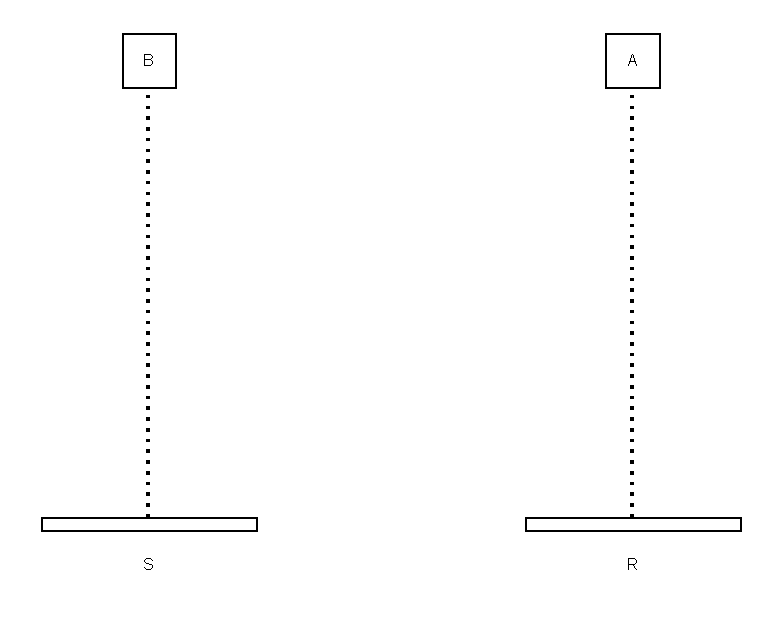
\includegraphics[width=0.6\textwidth]{scenario2a-setup-cropped.pdf}
	\caption{Two collinear rods moving towards each other, observers far away in perpendicular direction}
	\label{fig:scenario2a-setup}
\end{figure}

There is a person $A$ at rest relative to $R$, at a distance $D \gg L$
from the $R$'s center, at a direction $U$ perpendicular to $R$'s
length.  Rod $S$ is moving left to right with velocity $v$
($0 < v < c$) relative to $R$.  There is another person $B$ at rest
relative to $S$ at a distance $D$ from $S$'s center, in the same
direction $U$ from $S$'s center.

There are 3 events of interest, shown in Figure~\ref{fig:scenario2a-events}:
\begin{itemize}
\item Event 1: The left end of $R$ meets the right end of $S$.
\item Event 2: The left end of $R$ meets the left end of $S$.
\item Event 3: The right end of $R$ meets the right end of $S$.
\end{itemize}
In the figure, the location of each event is shown by a small circle
on the appropriate end of $R$.

\begin{figure}[ht]
	\centering
	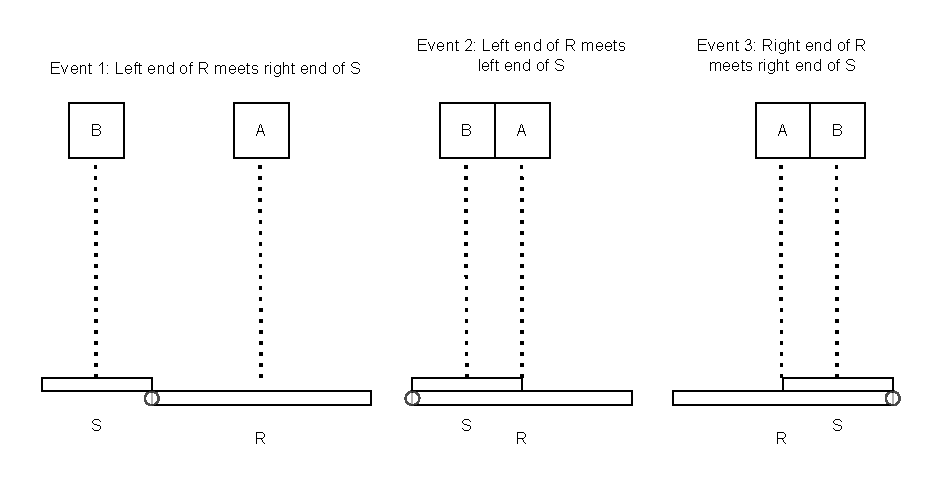
\includegraphics[width=1.0\textwidth]{scenario2a-events-cropped.pdf}
	\caption{Events of interest for Scenario 2a}
	\label{fig:scenario2a-events}
\end{figure}

Each of these events causes a light pulse to be emitted from the left
or right end of rod $R$, when the event is detected locally by some
devices built into the rods at each end.

The figure shows the order of events as observed by $A$ in $A$'s
frame.  The figure shows the moving rod $S$ contracts in length by a
large factor, to emphasize this.  We assume that the pulses can be
distinguished by $A$ in some way, e.g. by relative intensity,
frequency, and/or duration.

I have read that according to special relativity, because $D \gg L$,
the propagation time of the pulses from their sending points to $A$
should be effectively equal, and thus the relative order that $A$
receives the pulses is the same order that they are sent, and also the
difference in their arrival times should be equal to the difference in
their sending times.

In $A$'s frame, the sending times of the pulses are as follows.
(Detail: These equations can use $v$ instead of $|v|$ because
we are assuming $v > 0$.)
\begin{align*}
q_{1,A} & = 0 & & \text{for convenience as a starting time} \\
q_{2,A} & = \frac{L/\gamma}{v} & & \text{distance moved by $S$ since Event 1 is its contracted length} \\
q_{3,A} & = \frac{L}{v} & & \text{distance moved by $S$ since Event 1 is $R$'s rest length}
\end{align*}
Let $r_{1,A}, r_{2,A}, r_{3,A}$ be the times that $A$ measures for
receiving the 3 pulses.
\begin{align*}
r_{2,A} - r_{1,A} & = \frac{L}{\gamma v} & & \text{equal to $q_{2,A} - q_{1,A}$} \\
r_{3,A} - r_{1,A} & = \frac{L}{v} & & \text{equal to $q_{3,A} - q_{1,A}$}
\end{align*}

According to special relativity, if we calculate in $B$'s frame the
interval between $B$ receiving the pulses, we find that Event 3's
pulse reaches $B$ {\em before} Event 2's pulse, because in $B$'s frame, $S$
is its full rest length $L$, and $R$ is contracted in length.  So the
sequence of events is the ``mirror image'' of
Figure~\ref{fig:scenario2a-events}.

\begin{align*}
q_{1,B} & = 0 & & \text{see Note 1 below}\\
q_{2,B} & = \frac{L}{v} & & \text{distance moved by $R$ since Event 1 is $S$'s rest length} \\
q_{3,B} & = \frac{L/\gamma}{v} & & \text{distance moved by $R$ since Event 1 is its contracted length} \\
r_{2,B} - r_{1,B} & = \frac{L}{v} & & \text{equal to $q_{2,B} - q_{1,B}$} \\
r_{3,B} - r_{1,B} & = \frac{L}{\gamma v} & & \text{equal to $q_{3,B} - q_{1,B}$}
\end{align*}
Note 1: This is just a convenient starting time, with no attempt to
quantify any relationship between this and $q_{1,A}$.

Events 1 and 2 are timelike separated, because they are at the same
location, and one occurs earlier than the other.

Events 1 and 3 are timelike separated, because an object with mass
traveling at speed faster than $v$ relative to $A$, but less than $c$,
in the same direction as $S$'s velocity can move from event 1 to the
place where event 2 occurs, before event 2 occurs.

Events 2 and 3 are spacelike separated, because it would require
faster-than-light travel in $A$'s frame to move from the left end of
$R$ starting when event 2 occurs, to the right end of $R$ by the time
event 3 occurs.  As one example, note that rod $S$ in
Figure~\ref{fig:scenario2a-events} is drawn half the length of rod $R$,
so $\gamma=2$ in that figure.  This magnitude of length contraction
requires $v \approx 0.866c$.  Something would need to travel the
entire rest length of $R$ in the time it takes $S$ to move a distance
$0.5L$, i.e. it would need to move twice as fast as $S$, or $1.732c$
to reach the right end of $R$ before event 3 occurred.

Both in SR and LET, there are locations where an observer at rest
relative to $A$ will receive the pulses from event 2 before receiving
the pulse from event 3.  There are other locations where an observer
receives the pulses in the opposite order.  See the next section for
many details on this.

%TODO: Is there any subtle effect here if the pulses are emitted from a
%transmitter physically attached to rod $R$, versus attached to rod
%$S$?  For example, perhaps because the transmitters are moving at
%different velocities?
%
%Andy: I am fairly sure the answer is "no", so commenting this out for
%now.


\subsubsection{Where do observers at rest in $A$'s frame receive event 2 or 3 pulse first?}
\label{sec:scen2a-restpulsefirst}

For this section, assume either Special Relativity where rod $R$ and
observer $A$ are motionless with respect to us, or Lorentz Ether
Theory where they are motionless with respect to the ether.  Thus in
this section, light propagates in all directions with speed $c$.  For
SR, all times will be measured in $R$'s frame.  For LET, all times are
true times, as measured by clocks at rest relative to the ether.  We
will analyze more general situations later, if we can get a good
understanding of this one.

In scenario 2a, consider every location in the $XY$ plane.  A receiver
at rest relative to rod $R$ will receive the pulse from event 2 before
the pulse from event 3 in many locations, e.g. at the location of
event 2 at the left end of $R$.  Similarly, there are many locations
that will receive the event 3 pulse first, e.g. at the location of
event 3 at the right end of $R$.  There are also many locations that
receive both pulses at the same time.

What is the shape of all such places?

Let $R$'s left end be placed at coordinates $(-L/2,0)$ and its right
end at $(L/2,0)$.
As discussed in the previous section, the sending times of pulses for
events 1, 2, and 3 are as follows (we omit the $A$ in the subscripts
for brevity here);
\begin{align*}
q_1 & = 0 & & \text{for convenience as a starting time} \\
q_2 & = \frac{L/\gamma}{v} & & \text{distance moved by $S$ since Event 1 is its contracted length} \\
q_3 & = \frac{L}{v} & & \text{distance moved by $S$ since Event 1 is $R$'s rest length}
\end{align*}

At an arbitrary location $(x,y)$, it receives the pulse from event 2
at time $e_2$, and the pulse from event 3 at time $e_3$, given by:
\begin{align*}
e_2 & = q_2 + d_l/c & & \text{$d_l$ is distance between left end of $R$ and $(x,y)$} \\
e_3 & = q_3 + d_r/c & & \text{$d_r$ is distance between right end of $R$ and $(x,y)$}
\end{align*}
For a location that receives pulse 3 time $k$ later than receiving
pulse 2 (or before if $k < 0$) the following equation must be true:
\begin{align}
e_3 - e_2 & = k \nonumber \\
(q_3 + \frac{d_r}{c}) - (q_2 + \frac{d_l}{c}) & = k & & \text{defns. of $e_2, e_3$} \nonumber \\
d_r - d_l & = c (k - (q_3 - q_2)) & & \text{algebra} \label{eqn:pulserecvdiff1}
\end{align}
Below we derive equivalent formulas for $q_3 - q_2$:
\begin{align}
q_3 - q_2
  & = \frac{L}{v} - \frac{L}{\gamma v} & & \text{defns. of $q_2, q_3$} \nonumber \\
  & = \frac{L}{v} (1 - \frac{1}{\gamma}) & & \text{algebra} \nonumber \\
  & = \frac{L}{\beta c} (1 - \frac{1}{\gamma}) & & \text{replace $v$ with $\beta c$} \label{eqn:pulsesenddiff2} \\
  & = \frac{L}{c} \frac{\beta\gamma}{\gamma+1} & & \text{Lemma~\ref{lem:betaGammaIdentity1}} \label{eqn:pulsesenddiff}
\end{align}
The equivalent equation below is a bit easier to see the behavior as
$\beta$ approaches 0 or 1:
\begin{align*}
\frac{\beta\gamma}{\gamma+1} & = \beta(1-\frac{1}{\gamma+1})
\end{align*}
When $\beta$ approaches 0, this value approaches $0/2 = 0$.
When $\beta$ approaches 1, this value approaches $1(1-0) = 1$.
It is straightforward to verify by calculating the derivative that
this function is strictly increasing with $\beta$ over the interval $(0,1)$.

Substituting Equation~\eqref{eqn:pulsesenddiff} into
Equation~\eqref{eqn:pulserecvdiff1} gives:
\begin{align}
d_r - d_l
  & = c \left( k - \left( \frac{L}{c} \right) \frac{\beta\gamma}{\gamma+1} \right) \nonumber \\
  & = ck - \frac{L \beta \gamma}{\gamma+1}
\end{align}
If we restrict our attention to situations where $L$, $\beta$, and $k$
are given constants, this equation is of the form $d_r - d_l$ equal to
a constant.  The shape of all such curves is a
hyperbola~\cite{WikipediaHyperbolaDefnLocusOfPoints}.

Figure~\ref{fig:pulse-receive-deltas-L-1.0-beta-0.50} shows the $XY$
plane with $x$ and $y$ coordinates in units of light-seconds.  $L=1$
light-second, with rod $R$ parallel to the $x$ axis, centered at the
origin.  $\beta=0.5$ for this figure.
\begin{figure}[ht]
	\centering
	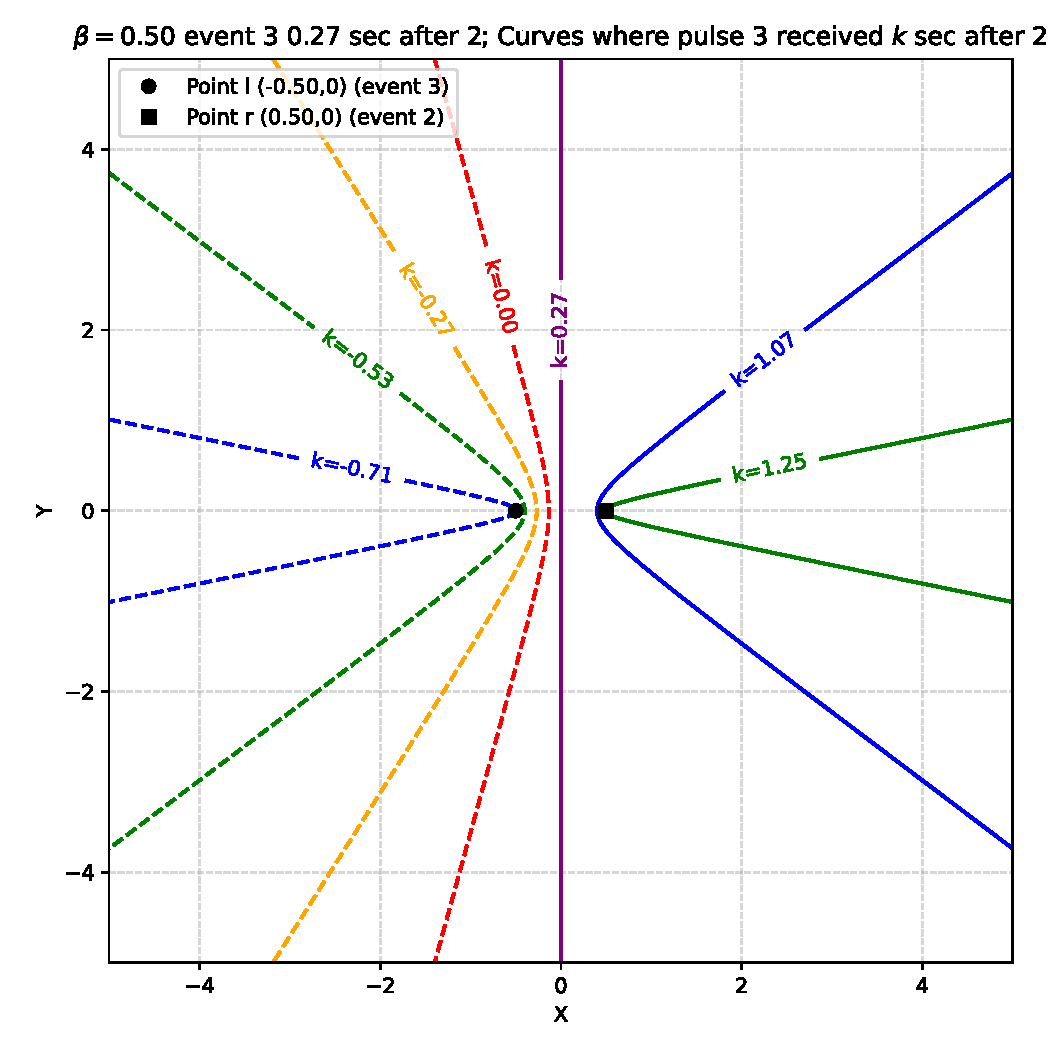
\includegraphics[width=1.0\textwidth]{pulse-receive-deltas-L-1.0-beta-0.50-cropped.pdf}
	\caption{Locations with selected values of $k$ for $\beta=0.5$, $q_3 - q_2 = 0.27$ sec}
	\label{fig:pulse-receive-deltas-L-1.0-beta-0.50}
\end{figure}
First consider the line labeled $k=0.27$ in the figure.  This is the
line where $k = q_3 - q_2$, so the pulse for event 3 arrives $k=0.27$
sec after the pulse for event 2.  This is exactly the difference in
times between when the pulses are generated, so this line is all of
the points equally distant in length from the two ends of rod $R$; a
vertical line along the $y$ axis.

Next consider the curve labeled $k=0$.  These are all locations where
the two pulses arrive simultaneously.  Since pulse 2 is sent 0.27 sec
earlier than pulse 3, all of these locations are 0.27 light-seconds
further from the left end of $R$ than from the right end.

The last curve we will give special attention to is the curve labeled
$k=-0.27$.  These are all locations where pulse 3 (emitted later),
arrives 0.27 {\em earlier} than pulse 2 (emitted earlier), which is
the relative order and separation in time that $B$ receives the pulses
according to SR.

For the line $y=D$ where $A$ and $B$ are located (far above the bounds
of the figure), $A$ is on the line $k=0.27$ at coordinates $(0, D)$.
But $B$ is moving to the right at speed $v$, so even though it is near
$A$ when the pulses are emitted, $B$ is a significant distance to the
right of $A$ when $B$ receives the pulses.  Is it so far to the right
that it is on the $k=-0.27$ line?

As we will show in the next section, $B$ reaches far enough to the
right that if you measure the difference in times that it receives the
pulses, according to time in $A$'s frame, and then multiply that by
$1/\gamma$ to account for $B$'s clock running slower than $A$'s clock,
the result is $-0.27$ sec.  And this correspondence is true for all
$\beta$ values, not only $\beta=0.5$ used in
Figure~\ref{fig:pulse-receive-deltas-L-1.0-beta-0.50}.


\subsubsection{Difference in time of pulses arriving to $B$, calculated in $A$'s frame}
\label{sec:scen2a-Breceivepulsetimes}

%We will make use of Lemma~\ref{lem:IntersectingSpreadingPulse} from
%Appendix~\ref{app:IntersectingSpreadingPulse} here.

For calculating when $B$ receives the pulses from events 2 and 3, it
is useful to know the location of $B$ at any time where it is
convenient to determine.  At the time of event 1 ($q_1=0$) the right
end of rod $S$ is at the same $x$ coordinate as the left end of rod
$R$, $x=-L/2$.  The center of rod $S$ is thus half of $S$'s contracted
length further to the left, at $x=-(L/2)(1+1/\gamma)$.  $B$'s $x$
coordinate is the same as the center of $S$ at all times.

\paragraph{Time when $B$ receives pulse from event 2}

Note that this time is calculated in $R$'s frame.
In the notation of Lemma~\ref{lem:IntersectingSpreadingPulse}:
\begin{align*}
\vect{s} & = (-L/2, 0) & & \text{pulse sent from $\vect{s}$, location of event 2} \\
t_0 & = \frac{L}{\gamma v} & & \text{pulse sent at time $t_0$, time of event 2} \\
\vect{s} + \vect{r}_1 & = ((-L/2)(1+1/\gamma), D) & & \text{$\vect{s}+\vect{r}_1$ is location of $B$ at time $t_1=0$} \\
\vect{r}_1 & = (-L/(2 \gamma), D) & & \text{subtract $\vect{s}$ from previous line to get $\vect{r}_1$} \\
\vect{r}_0 & = \vect{r}_1 + \vect{v}(t_0-t_1) \\
           & = (-L/(2 \gamma) + vL/(\gamma v), D) \\
           & = (L/(2 \gamma), D)
\end{align*}
The result of Lemma~\ref{lem:IntersectingSpreadingPulse} gives us the
time (in $R$'s frame) when $B$ receives the event 2 pulse:
\begin{equation}
  e_2 = \frac{L}{\gamma v} +
        \frac{\gamma^2}{c^2} \left[ \frac{Lv}{2 \gamma} + \sqrt{ \frac{L^2v^2}{4 \gamma^2} + (1-\beta^2)c^2 (\frac{L^2}{4 \gamma^2} + D^2) } \right]
\label{eqn:Breceivespulse2}
\end{equation}

\paragraph{Time when $B$ receives pulse from event 3}

This is very similar to the calculation for event 2.
Again in the notation of Lemma~\ref{lem:IntersectingSpreadingPulse}:
\begin{align*}
\vect{s} & = (L/2, 0) & & \text{pulse sent from $\vect{s}$, location of event 3} \\
t_0 & = \frac{L}{v} & & \text{pulse sent at time $t_0$, time of event 3} \\
\vect{s} + \vect{r}_1 & = ((-L/2)(1+1/\gamma), D) & & \text{$\vect{s}+\vect{r}_1$ is location of $B$ at time $t_1=0$, same as above} \\
\vect{r}_1 & = (-L - L/(2 \gamma), D) & & \text{subtract $\vect{s}$ from previous line to get $\vect{r}_1$} \\
\vect{r}_0 & = \vect{r}_1 + \vect{v}(t_0-t_1) \\
           & = (-L - L/(2 \gamma) + vL/v, D) \\
           & = (-L/(2 \gamma), D)
\end{align*}
The result of Lemma~\ref{lem:IntersectingSpreadingPulse} gives us the
time (in $R$'s frame) when $B$ receives the event 3 pulse:
\begin{equation}
  e_3 = \frac{L}{v} +
        \frac{\gamma^2}{c^2} \left[ -\frac{Lv}{2 \gamma} + \sqrt{ \frac{L^2v^2}{4 \gamma^2} + (1-\beta^2)c^2 (\frac{L^2}{4 \gamma^2} + D^2) } \right]
\label{eqn:Breceivespulse3}
\end{equation}

\paragraph{Relative time when $B$ receives pulses from events 2 and 3}

It is convenient that the subexpressions of
Equations~\eqref{eqn:Breceivespulse2} and~\eqref{eqn:Breceivespulse3}
under the radicals are equal, so they cancel out when we determine
$e_3 - e_2$, resulting in:
\begin{align}
e_3 - e_2
  & = \frac{L}{v}(1-\frac{1}{\gamma}) + \frac{\gamma^2}{c^2} \left[ -\frac{Lv}{2 \gamma} - \frac{Lv}{2 \gamma} \right] \nonumber \\
  & = \frac{L}{v}(1-\frac{1}{\gamma}) - \frac{\gamma Lv}{c^2} & & \text{algebra} \nonumber \\
  & = \frac{L}{\beta c}(1-\frac{1}{\gamma}) - \frac{\gamma L\beta}{c} & & \text{replace $v$ with $\beta c$ and algebra} \nonumber \\
  & = \frac{L}{c} \left[ \frac{1}{\beta}(1-\frac{1}{\gamma}) - \beta \gamma \right] & & \text{algebra} \nonumber \\
  & = \frac{L}{c} \left( \frac{\beta\gamma}{\gamma+1} - \beta \gamma \right) & & \text{Lemma~\ref{lem:betaGammaIdentity1}} \nonumber \\
  & = \frac{L\beta\gamma}{c} \left( \frac{1}{\gamma+1} - 1 \right) & & \text{algebra} \nonumber \\
  & = \frac{L\beta\gamma}{c} \left( \frac{-\gamma}{\gamma+1} \right) & & \text{algebra} \nonumber \\
  & = - \frac{L}{c} \left( \frac{\beta\gamma^2}{\gamma+1} \right) & & \text{algebra} \label{eqn:Bdeltatime3minus2}
\end{align}

We want to show that when we convert this difference $e_3 - e_2$ into
$B$'s slower-running clock, by multiplying by $1/\gamma$, we get the
{\em negative} of $q_3 - q_2$, where $q_3 - q_2$ is the (positive)
time that event 3's pulse is sent after event 2's pulse is sent, in
$A$'s frame.

\begin{align*}
\frac{1}{\gamma}(e_3 - e_2)
  & = - \frac{L}{\gamma c} \left( \frac{\beta\gamma^2}{\gamma+1} \right) & & \text{Eqn.~\eqref{eqn:Bdeltatime3minus2}} \\
  & = - \frac{L}{c} \left( \frac{\beta\gamma}{\gamma+1} \right) & & \text{algebra} \\
  & = - (q_3 - q_2) & & \text{Eqn.~\eqref{eqn:pulsesenddiff}}
\end{align*}


\subsection{Special Relativity Scenario 2b: Two rods moving towards each other at constant velocity, and both relative to observer}
\label{sec:scen2b}

Scenario 2b is a small generalization of Scenario 2a.  The intent in
doing this is that in LET, if $A$ and $B$ do not know their motion
relative to the ether, the results in this section will show what they
will be able to observe and measure, for at least some kinds of motion
of both of them relative to the ether, while they only directly
observe their uniform constant motion to each other and the rods.

TODO: It would be nice to generalize this further to $A$ and $B$ at
uniform speed motion towards each other, but they both have an
arbitrary 2-dimensional velocity vector $\vect v = (v_x, v_y)$ in the
$XY$ plane.

The only differences between Scenario 2b and Scenario 2a are that rod
$R$ and $A$ are moving parallel to the $x$ direction with velocity
$v_R$.  The velocity of $S$ and $B$ is denoted $v_S$ to distinguish it
from $v_R$.

$S$ starts at a lesser $x$ coordinate than $R$.  We want $S$ to catch
up to $R$, so we only consider $v_S > v_R$.  We also want $S$ to be
length-contracted to a shorter length than $R$, to make it similar to
Scenario 2a and reduce the number of cases to consider, so we only
consider $|v_S| > |v_R|$.

All calculations are done in the rest frame, except for conversion of
time intervals to/from $A$ and $B$'s frame as near to the beginning or
end of the calculation as possible.  This keeps all calculations
consistent with LET in the rest frame, or SR in the frame of a new
observer $O$ with velocity 0.

$R$ is contracted to length $L/\gamma_{R}$,
and $S$ is contracted to length $L/\gamma_{S}$.
Events 1, 2, and 3 are the same as in Scenario 2a.
\begin{align}
x_R(t) & = x_{R,0} + v_R t & & \text{$x_R(t)$ is $x$ coordinate of $R$'s center at time $t$} \\
x_S(t) & = x_{S,0} + v_S t & & \text{$x_S(t)$ is $x$ coordinate of $S$'s center at time $t$}
\end{align}

The details of the calculations are in Appendix~\ref{app:scen2b}.
They are very similar to those for Scenario 2a.

The result is that the times $e_{2,A}$ and $e_{3,A}$ when $A$ receives
the pulses from event 2 and 3, as measured in the rest frame, differ
by the following (a positive value, since $A$ receives the pulse for
event 2 before the pulse for event 3):
\begin{equation}
e_{3,A}-e_{2,A}
  = \frac{\gamma_R L}{c} \left[ \frac{\beta_S\gamma_S - \beta_R\gamma_R}{\gamma_S + \gamma_R} \right] \label{eqn:scen2b-pulseReceiveDiffForA}
\end{equation}

The times $e_{2,B}$ and $e_{3,B}$ when $B$ receives the pulses, as
measured in the rest frame, differ by the following (a negative value,
since $B$ receives the pulse for event 3 before the pulse for event
2):
\begin{equation}
e_{3,B}-e_{2,B}
  = -\frac{\gamma_S L}{c} \left[ \frac{\beta_S\gamma_S - \beta_R\gamma_R}{\gamma_S + \gamma_R} \right] \label{eqn:scen2b-pulseReceiveDiffForB}
\end{equation}

The difference between receiving the pulses as measured on $A$'s
slower clock is $1/\gamma_R$ times
Equation~\eqref{eqn:scen2b-pulseReceiveDiffForA}.  Similarly the
difference between receiving the pulses as measured on $B$'s slower
clock is $1/\gamma_S$ times
Equation~\eqref{eqn:scen2b-pulseReceiveDiffForB}.  It is easily seen
from the equations above that:
\begin{equation}
\frac{1}{\gamma_R} (e_{3,A}-e_{2,A}) = -\frac{1}{\gamma_S} (e_{3,B}-e_{2,B})
\end{equation}

Similar to what was described at the end of
Section~\ref{sec:scen1b-BtoCLETfriendly} for Scenario 1b, where $B$ and
$C$, both in motion relative to $A$, get measurements consistent with
$B$ being at rest and $C$ having relative velocity equal to $v_C
\ominus v_B$ relative to $B$ (or $C$ at rest and $B$ having relative
velocity $v_B \ominus v_C$ relative to $C$), there is a similar result
here.

The difference in time measured by $A$ on its local clock of the two
pulses is:
\begin{align*}
\frac{1}{\gamma_R} (e_{3,A}-e_{2,A})
  = \frac{L}{c} \left[ \frac{\beta_S\gamma_S - \beta_R\gamma_R}{\gamma_S + \gamma_R} \right] & & \text{Eqn.~\eqref{eqn:scen2b-pulseReceiveDiffForA}} \\
  = \frac{L}{c} \tanh \frac{\eta_S-\eta_R}{2} & & \text{Lemma~\ref{lem:halfRapidityDifference} in Appendix~\ref{app:1drelVelocityUsingHyperbolicFns}} \\
  = \frac{L}{c} \tanh \frac{\eta_{\Delta}}{2} & & \text{define $\eta_{\Delta}=\eta_S-\eta_R$}
\end{align*}
where $\eta_S = \tanh^{-1} \beta_S$ and $\eta_R = \tanh^{-1} \beta_R$.
The rapidity value $\eta_{\Delta}$ corresponds to the relativistic
velocity $\beta_{\Delta} = \beta_S \ominus \beta_R$.  Thus as long as
$A$ knows $L$, it can calculate a value of $\beta_{\Delta}$ from
its measured difference between the pulse arrival times $T$:
\begin{align}
T & = \frac{L}{c} \tanh \frac{\eta_{\Delta}}{2} & & \text{from above} \nonumber \\
\tanh \frac{\eta_{\Delta}}{2} & = \frac{cT}{L} & & \text{algebra} \label{eqn:tanhOfHalfEtaDelta}
\end{align}
then:
\begin{align*}
\beta_{\Delta}
  & = \tanh \eta_{\Delta} & & \text{relationship between $\beta$ and $\eta$ Eqn.~\eqref{eqn:betaHyperbolic}} \\
  & = \frac{2\tanh \frac{\eta_{\Delta}}{2}}{1+\tanh^2 \frac{\eta_{\Delta}}{2}} & & \text{Eqn.~\eqref{eqn:tanhDoubleAngle}} \\
  & = \frac{2 (\frac{cT}{L})}{1+(\frac{cT}{L})^2} & & \text{Eqn.~\eqref{eqn:tanhOfHalfEtaDelta}} \\
\end{align*}
$B$ measures exactly the negative of the time difference, and
following the same kinds of calculations can calculate the negative of
$\beta_{\Delta}$ that $A$ does.


%\newpage
\bibliography{refs}

\appendix

\section{Miscellaneous math facts}

\subsection{Math facts about relativistic velocity addition and subtraction in one dimension}
\label{app:1drelvelocityadd}

All of the facts here are quite simple to validate.  I write them out
primarily as an aid to thinking about and remembering them, and they
might also be useful to refer to from elsewhere in this document.

Note that this appendix is restricted to proofs of simple mathematical
relationships about the definitions of one-dimensional relativistic
velocity addition and subtraction formulas.  This appendix makes no
claims about the physical meaning of these operations.

I have read that relativistic velocity addition in 3 dimensions is not
associative.  TODO: If I add any discussion of 3-dimensional
relativity examples to this document, it would be nice to give an
example, perhaps in a separate appendix.

In one dimension, though, all velocities of subliminal entities can be
represented by $v$ such that $-c < v < c$, where negative velocities
are in the opposite direction along the line than positive velocities.

The can also be represented as relativistic velocity $\beta = v/c$,
i.e. a fraction of $c$.  These are in the range $-1 < \beta < 1$.

I will use the notation $v \oplus w$ for relativistic velocity
addition.  While I will use the same symbol $\beta_v \oplus \beta_w$
for relativistic velocity addition of relativistic velocity values,
one should be careful to note that the definition of the operator
$\oplus$ is slightly different for these two cases.

\begin{align}
v \oplus w & = \frac{v+w}{1+\frac{vw}{c^2}} \label{defn:reladd1} \\
v \ominus w & = \frac{v-w}{1-\frac{vw}{c^2}} \label{defn:relsub1} \\
\beta_v \oplus \beta_w & = \frac{\beta_v+\beta_w}{1+\beta_v \beta_w} \label{defn:reladd2} \\
\beta_v \ominus \beta_w & = \frac{\beta_v-\beta_w}{1- \beta_v \beta_w} \label{defn:relsub2}
\end{align}

The proofs are only given for the relativistic velocity
formulas~\eqref{defn:reladd2} and~\eqref{defn:relsub2}.  The proofs
for equations~\eqref{defn:reladd1}
and~\eqref{defn:relsub1} are nearly identical.

We will use the symbols $a, b, c$ to represent arbitrary real values
between -1 and 1, to avoid writing $\beta$ with subscripts all over
the place.

\begin{align}
a \oplus b & = b \oplus a & & \text{addition is commutative (1-d only, not 3-d!)} \label{defn:1dreladdcommutative} \\
(a \oplus b) \oplus c & = a \oplus (b \oplus c) & & \text{addition is associative (1-d only, not 3-d!)} \label{defn:1dreladdassociative} \\
a \oplus 0 & = 0 \oplus a = a \\
a \oplus (-b) & = a \ominus b \\
a \ominus (-b) & = a \oplus b \\
0 \ominus b & = -b \\
a \ominus b & = - (b \ominus a)
\end{align}
The following inequalities only hold if $0 < a < 1$ and $0 < b < 1$:
\begin{align}
a \oplus b & > a \label{inequal:reladdposlarger1} \\
a \oplus b & > b \label{inequal:reladdposlarger2} \\
a \oplus b & < a+b \label{inequal:reladdpossmallerthansum}
\end{align}
The following inequality holds for all $-1 < a < 1$ and $-1 < b < 1$:
\begin{align}
-1 < a \oplus b & < 1 \label{inequal:reladdpossmallerthanc}
\end{align}
The last one is only slightly different if we use velocity addition on
normal velocities, i.e. velocities that are not relativistic velocities,
where $-c < v < c$ and $-c < w < c$:
\begin{align}
-c < v \oplus w & < c \label{inequal:reladdpossmallerthanc2}
\end{align}
The inequalities all have examples where the two sides can be very
nearly equal, such as these:
\begin{align*}
0.1 \oplus 0.001 & \approx 0.100989901 > 0.1 \\
0.1 \oplus 0.1 & \approx 0.198019802 < 0.1+0.1 \\
0.99 \oplus 0.99 & \approx 0.999949498 < 1
\end{align*}

Proving most of these is as simple as substituting the definition of
$a \oplus b$ and $a \ominus b$, and a tiny amount of algebra.

Proving associativity~\eqref{defn:1dreladdassociative} is only a
little bit more algebra, but we will do the steps here:
\begin{align*}
(a \oplus b) \oplus c
  & = \frac{\frac{a+b}{1+ab}+c}{1+\left(\frac{a+b}{1+ab}\right)c} & & \text{use Defn.~\eqref{defn:reladd2} twice} \\
  & = \frac{(a+b)+c(1+ab)}{(1+ab)+(a+b)c} & & \text{multiply numerator and denominator by $(1+ab)$} \\
  & = \frac{a+b+c+abc}{1+ab+ac+bc} & & \text{multiply out the terms}
\end{align*}
Similarly:
\begin{align*}
a \oplus (b \oplus c)
  & = \frac{a+\frac{b+c}{1+bc}}{1+a\left(\frac{b+c}{1+bc}\right)} & & \text{use Defn.~\eqref{defn:reladd2} twice} \\
  & = \frac{a(1+bc)+(b+c)}{(1+bc)+a(b+c)} & & \text{multiply numerator and denominator by $(1+bc)$} \\
  & = \frac{a+abc+b+c}{1+bc+ab+ac} & & \text{multiply out the terms}
\end{align*}
The above two final results are easily seen to be equal.

The inequalities are also not difficult to prove, but we will write
out their short proofs.  Recall that these inequalities are true only
for $0 < a < 1$ and $0 < b < 1$.  Similar inequality hold if both $a$
and $b$ are negative.

For the proof of inequality~\eqref{inequal:reladdposlarger1}, recall
that we can multiply or divide both sides of an inequality by the same
positive number, and the resulting inequality is true if and only if
the original one was.  The symbol $\Leftrightarrow$ below means ``if
and only if'', i.e. the expression before is true if and only if the
expression after is true.
\begin{align*}
a < \frac{a+b}{1+ab}
  & \Leftrightarrow a + a^2 b < a+b & & \text{multiply both sides by $1+ab$, which is positive} \\
  & \Leftrightarrow a^2 b < b & & \text{subtract $a$ from both sides} \\
  & \Leftrightarrow a^2 < 1 & & \text{divide both sides by $b$, which is positive}
\end{align*}
The last inequality is true because $a < 1$.
The proof of inequality~\eqref{inequal:reladdposlarger2} is the same
as above.

To prove $a \oplus b < a+b$
(inequality~\eqref{inequal:reladdpossmallerthansum}):
\begin{align*}
\frac{a+b}{1+ab} < a+b
  & \Leftrightarrow a+b < (a+b)(1+ab) & & \text{multiply both sides by $1+ab$, which is positive} \\
  & \Leftrightarrow 1 < (1+ab) & & \text{divide both sides by $a+b$, which is positive} \\
  & \Leftrightarrow 0 < ab & & \text{subtract 1 from both sides}
\end{align*}
The final inequality is true because both $a$ and $b$ are positive.

Now to prove $a \oplus b < 1$ (part of
inequality~\eqref{inequal:reladdpossmallerthanc}), but recall now we
are doing so for the more general case of all values $-1 < a < 1$ and
$-1 < b < 1$:
\begin{align*}
\frac{a+b}{1+ab} < 1
  & \Leftrightarrow a+b < 1+ab & & \text{multiply both sides by $1+ab$, which is positive} \\
  & \Leftrightarrow b-ab < 1-a & & \text{subtract $a+ab$ from both sides} \\
  & \Leftrightarrow b(1-a) < 1-a & & \text{algebra} \\
  & \Leftrightarrow b < 1 & & \text{divide both sides by $1-a$, which is positive}
\end{align*}
And the last inequality is true.  Proving the part that

\begin{align*}
-1 < \frac{a+b}{1+ab}
  & \Leftrightarrow -(1+ab) < a+b & & \text{multiply both sides by $1+ab$, which is positive} \\
  & \Leftrightarrow -(1+a) < b+ab & & \text{add $ab-a$ to both sides} \\
  & \Leftrightarrow -(1+a) < b(1+a) & & \text{algebra} \\
  & \Leftrightarrow -1 < b & & \text{divide both sides by $1+a$, which is positive}
\end{align*}
And the last inequality is true.


\subsection{Using hyperbolic functions for relativistic velocity arithmetic in one dimension}
\label{app:1drelVelocityUsingHyperbolicFns}

Logarithms and exponential functions are well known for the following
properties:
\begin{align*}
l & = \log_{10} x \\
x & = 10^l \\
l_3 = l_1 + l_2 & \Leftrightarrow x_3 = x_1 x_2 & & \text{$+$ of logs corresponds to multiplication of numbers} \\
l_3 = l_1 - l_2 & \Leftrightarrow x_3 = x_1 / x_2 & & \text{$-$ of logs corresponds to division of numbers} \\
l_3 = c l_1 & \Leftrightarrow x_3 = x_1^c & & \text{multiplying log by constant corresponds to exponentiation of numbers} \\
l_3 = l_1/c & \Leftrightarrow x_3 = x_1^{1/c} & & \text{dividing log by constant corresponds to taking $c$-th root of numbers} \\
\end{align*}

Hyperbolic functions~\cite{WikipediaHyperbolicFunctions} have a
similar correspondence to relativistic velocities $\beta$ and related
quantities like the Lorentz factor $\gamma$.
\begin{align}
\eta & = \tanh^{-1} \beta & & \text{calculate the {\em rapidity} $\eta$ from relativistic velocity} \\
\beta & = \tanh \eta & & \text{get $\beta$ from rapidity} \label{eqn:betaHyperbolic} \\
\gamma & = \cosh \eta & & \text{get $\gamma$ from rapidity} \label{eqn:gammaHyperbolic} \\
D & = \sqrt{\frac{1+\beta}{1-\beta}} = e^\eta & & \text{get Doppler factor from rapidity} \label{eqn:dopplerFactorHyperbolic} \\
\beta \gamma & = \sinh \eta & & \text{get $\beta \gamma$ from rapidity} \label{eqn:betaGammaHyperbolic} \\
\eta_3 = \eta_1 + \eta_2 & \Leftrightarrow \beta_3 = \beta_1 \oplus \beta_2 & & \text{$+$ of rapidity corresponds to 1-d relativistic velocity $\oplus$} \\
    & \Leftrightarrow D_3 = D_1 D_2 & & \text{and to 1-d Doppler factor multiplication} \\
\eta_3 = \eta_1 - \eta_2 & \Leftrightarrow \beta_3 = \beta_1 \ominus \beta_2 & & \text{$-$ of rapidity corresponds to 1-d relativistic velocity $\ominus$} \\
    & \Leftrightarrow D_3 = D_1 / D_2 & & \text{and to 1-d Doppler factor division} \\
\end{align}
Also:
\begin{itemize}
\item Multiplying a rapidity by a positive number $n$ corresponds to
  repeatedly adding that relativistic velocity $n$ times.
\item Dividing a rapidity by a positive number $n$ corresponds to
  finding a relativistic velocity $\beta$ such that repeated velocity
  addition of $\beta$ $n$ times will give back the original
  relativistic velocity.
\end{itemize}
There are an abundance of identities involving hyperbolic functions,
similar to the large variety of identities relating trigonometric
functions.  These identities can be useful for finding relationships
between relativistic $\beta$ and $\gamma$ values.

Examples of a few hyperbolic function identities, but there are many
more~\cite{WikipediaHyperbolicFunctions}:
\begin{align}
\sinh (-x) & = -\sinh x \\
\cosh (-x) & = \cosh x \\
\tanh (-x) & = - \tanh x \\
\sinh (x \pm y) & = \sinh x \cosh y \mp \cosh x \sinh y \\
\cosh (x \pm y) & = \cosh x \cosh y \pm \sinh x \sinh y \\
\tanh (x \pm y) & = \frac{\tanh x \pm \tanh y}{1 \pm \tanh x \tanh y} \\
\sinh x + \sinh y & = 2 \sinh (\frac{x+y}{2} ) \cosh (\frac{x-y}{2}) \label{eqn:sinhHalfAngleSum} \\
\cosh x + \cosh y & = 2 \cosh (\frac{x+y}{2} ) \cosh (\frac{x-y}{2}) \label{eqn:coshHalfAngleSum} \\
\tanh 2x & = \frac{2 \tanh x}{1+\tanh^2 x} \label{eqn:tanhDoubleAngle}
\end{align}

Below are a couple of examples of the use of hyperbolic functions,
relevant elsewhere in this document, that I have personally found much
more difficult to validate without using hyperbolic functions.

\begin{lemma}
\label{lem:halfRapidityDifference}
Let $\beta_1, \beta_1$ be any real values in the range $(-1,1)$,
$\gamma_1, \gamma_1$ their corresponding Lorentz factors, and $\eta_i
= \tanh^{-1} \beta_i$ their rapidities.
Then:
\begin{equation}
\frac{\beta_1 \gamma_1 - \beta_2 \gamma_2}{\gamma_1 + \gamma_2} = \tanh \frac{\eta_1-\eta_2}{2}
\end{equation}
\end{lemma}

\begin{proof}
\begin{align*}
\frac{\beta_1 \gamma_1 - \beta_2 \gamma_2}{\gamma_1 + \gamma_2}
  & = \frac{\sinh \eta_1 - \sinh \eta_2}{\cosh \eta_1 + \cosh \eta_2} & & \text{Eqns.~\eqref{eqn:betaGammaHyperbolic} and~\eqref{eqn:gammaHyperbolic}} \\
  & = \frac{2 \sinh ( \frac{\eta_1-\eta_2}{2} ) \cosh ( \frac{\eta_1+\eta_2}{2} ) }{2 \cosh ( \frac{\eta_1+\eta_2}{2} ) \cosh ( \frac{\eta_1-\eta_2}{2} ) } & & \text{Eqns.~\eqref{eqn:sinhHalfAngleSum} and~\eqref{eqn:coshHalfAngleSum}} \\
  & = \frac{\sinh ( \frac{\eta_1-\eta_2}{2} ) }{\cosh ( \frac{\eta_1-\eta_2}{2} ) } & & \text{cancel common terms} \\
  & = \tanh \frac{\eta_1-\eta_2}{2} & & \text{$\tanh x = \sinh x / \cosh x$}
\end{align*}
\end{proof}

\begin{corollary}
Let $\beta$ be any real value in the range $(-1,1)$, $\gamma$ its
corresponding Lorentz factor, and $\eta = \tanh^{-1} \beta$ its
rapidity.
Then:
\begin{equation}
\frac{\beta \gamma}{\gamma + 1} = \tanh \frac{\eta}{2}
\end{equation}
\end{corollary}

\begin{proof}
Follows directly from Lemma~\ref{lem:halfRapidityDifference} by
substituting $\beta_2 =0$, from which follows $\gamma_2 = 1$ and
$\eta_2=0$.
\end{proof}


\subsection{Relativistic velocity addition and subtraction in 3 dimensions}
\label{app:3drelvelocityaddsub}


\subsubsection{Decomposing vector $\vect{u}$ into components parallel and perpendicular to vector $\vect{v}$}
\label{app:decomposeVectorIntoParallelPlusPerpendicular}

Sometimes it can be useful to take vectors $\vect{u}$ and $\vect{v}$,
and express $\vect{u}$ as a sum of two vectors $\vect{u}_{\parallel}$
and $\vect{u}_{\perp}$ that satisfy these conditions:
\begin{itemize}
\item $\vect{u} = \vect{u}_{\parallel} + \vect{u}_{\perp}$
\item $\vect{u}_{\parallel}$ is parallel to $\vect{v}$.
\item $\vect{u}_{\perp}$ is perpendicular to $\vect{v}$,
  i.e. $\vect{u}_{\perp} \cdot \vect{v} = 0$.
\end{itemize}

The direction of $\vect{u}_{\parallel}$ is parallel to $\vect{v}$.
The magnitude of $\vect{u}_{\parallel}$ is the portion of $\vect{u}$'s
magnitude that is parallel to $\vect{v}$, which is $u \cos \theta$,
where $\theta$ is the angle between $\vect{u}$ and $\vect{v}$.
\begin{align}
\vect{u}_{\parallel}
  & = (\text{unit vector in direction of $\vect{v}$})(\text{magnitude of $\vect{u}_{\parallel}$}) \nonumber \\
  & = (\frac{\vect{v}}{v}) (u \cos \theta) \nonumber \\
  & = (\frac{\vect{v}}{v}) (u \frac{\vect{u} \cdot \vect{v}}{uv}) & & \text{$\vect{u} \cdot \vect{v} = uv \cos \theta$} \nonumber \\
  & = (\frac{\vect{v}}{v^2}) (\vect{u} \cdot \vect{v}) & & \text{algebra} \nonumber \\
\vect{u}_{\parallel}
  & = \frac{\vect{u} \cdot \vect{v}}{v^2} \vect{v} & & \text{algebra} \label{eqn:uParallel}
\end{align}

This vector equation turns out to be useful in finding an equation for
$\vect{u}_{\perp}$ in other forms:
\begin{equation}
(\vect{u} \times \vect{v}) \times \vect{v} = (\vect{u} \cdot \vect{v}) \vect{v} - v^2 \vect{u} \label{eqn:2CrossProductsIdentity}
\end{equation}
Divide both sides of that equation by $v^2$ and rearrange a bit to get:
\begin{equation}
\frac{(\vect{u} \cdot \vect{v})}{v^2} \vect{v} = \frac{1}{v^2} (\vect{u} \times \vect{v}) \times \vect{v} + \vect{u} \label{eqn:2CrossProductsIdentityRearranged}
\end{equation}
\begin{align}
\vect{u} & = \vect{u}_{\parallel} + \vect{u}_{\perp} \nonumber \\
\vect{u}_{\perp}
  & = \vect{u} - \vect{u}_{\parallel} & & \text{algebra} \nonumber \\
  & = \vect{u} - \frac{\vect{u} \cdot \vect{v}}{v^2} \vect{v} & & \text{Eqn.~\eqref{eqn:uParallel}} \nonumber \\
  & = \vect{u} - (\frac{1}{v^2} (\vect{u} \times \vect{v}) \times \vect{v} + \vect{u}) & & \text{Eqn.~\eqref{eqn:2CrossProductsIdentityRearranged}} \nonumber \\\vect{u}_{\perp}
  & = - \frac{1}{v^2} (\vect{u} \times \vect{v}) \times \vect{v} & & \text{algebra} \label{eqn:uPerpendicular}
\end{align}


\subsubsection{Relativistic velocity addition in 3 dimensions}
\label{app:3drelvelocityadd}

Let:
\begin{align*}
  \vect{v}_B & & \text{velocity of frame $B$ relative to frame $A$} \\
  \vect{u}' & & \text{velocity of object in frame $B$} \\
  \vect{v}_A & & \text{velocity of object in frame $A$}
\end{align*}
\begin{align}
\vect{v}_A = \vect{v}_B \oplus \vect{u}'
  & = \frac{ \vect{u}' + \left[ (\gamma_B-1) \frac{\vect{v}_B \cdot \vect{u}'}{v_B^2} + \gamma_B \right] \vect{v}_B }
           { \gamma_B (1 + \frac{\vect{v}_B \cdot \vect{u}'}{c^2}) } & & \text{\cite{WikipediaVelocityAdditionFormula}} \label{eqn:relVelocityAdd1} \\
  & = \frac{ \vect{v}_B + \vect{u}' + \frac{\gamma_B}{\gamma_B+1} (\vect{u}' \times \vect{v}_B) \times \vect{v}_B / c^2 }
           { 1 + \frac{\vect{v}_B \cdot \vect{u}'}{c^2} } \label{eqn:relVelocityAdd2} \\
  & = \vect{v}_{A \parallel} + \vect{v}_{A \perp} \label{eqn:relVelocityAddComponents}
\end{align}
where:
\begin{align}
\vect{v}_{A \parallel}
  & = \frac{ \vect{v}_B + \vect{u}'_{\parallel} }{1 + \frac{ \vect{v}_B \cdot \vect{u}'}{c^2} } \label{eqn:relVelocityAddParallelComponent} \\
\vect{v}_{A \perp}
  & = \frac{ \vect{u}'_{\perp} }{\gamma_B (1 + \frac{ \vect{v}_B \cdot \vect{u}'}{c^2} )} \label{eqn:relVelocityAddPerpendicularComponent}
\end{align}
and formulas for $\vect{u}'_{\parallel}$ and $\vect{u}'_{\perp}$ can
be found in the previous section.  It is only a few steps of algebra
to plug Equations~\eqref{eqn:relVelocityAddParallelComponent}
and~\eqref{eqn:relVelocityAddPerpendicularComponent}
into~\eqref{eqn:relVelocityAddComponents} and show it is equal
to~\eqref{eqn:relVelocityAdd1}, so we will not do so here.
Similarly, it is not many steps to show that
Equations~\eqref{eqn:relVelocityAdd1} and~\eqref{eqn:relVelocityAdd2}
are equal, using~\eqref{eqn:uPerpendicular}.

Relativistic velocity subtraction:
\begin{align}
\vect{u}' = \vect{v}_A \ominus \vect{v}_B
  & = \frac{ \vect{v}_A - \vect{v}_B + \frac{\gamma_B}{\gamma_B+1} (\vect{v}_A \times \vect{v}_B) \times \vect{v}_B / c^2 }
           { 1 - \frac{\vect{v}_A \cdot \vect{v}_B}{c^2} } & & \text{\cite{Koczan2021}} \\
  & = \vect{u}'_{\parallel} + \vect{u}'_{\perp} \label{eqn:relVelocitySubComponents}
\end{align}
where:
\begin{align}
\vect{u}'_{\parallel}
  & = \frac{ \vect{v}_{A \parallel} - \vect{v}_B}{1 - \frac{ \vect{v}_A \cdot \vect{v}_B}{c^2} } \label{eqn:relVelocitySubParallelComponent} \\
\vect{u}'_{\perp}
  & = \frac{ \vect{v}_{A \perp} }{\gamma_B (1 - \frac{ \vect{v}_A \cdot \vect{v}_B}{c^2} )} \label{eqn:relVelocitySubPerpendicularComponent}
\end{align}

I was able to get Mathematica to confirm that
for all vectors $\vect{v}_B$, $\vect{u}'$:
\begin{equation}
(\vect{v}_B \oplus \vect{u}') \ominus \vect{v}_B = \vect{u}'
\end{equation}
Similarly for all vectors $\vect{v}_A$, $\vect{v}_B$:
\begin{equation}
\vect{v}_B \oplus (\vect{v}_A \ominus \vect{v}_B) = \vect{v}_A
\end{equation}


\subsection{Math facts about the Doppler factor and Lorentz factor}
\label{app:DopplerFactor}

This appendix is restricted to proofs of mathematical relationships.
It makes no claims about the physical meaning of the equations
involved.

Define $D$ as given by Definition~\eqref{defn:DopplerFactor}, repeated
here:
\begin{align*}
D & = \sqrt{ \frac{1 + \beta}{1 - \beta} } & & \text{Repeat of Defn.~\eqref{defn:DopplerFactor}}
\end{align*}
Define it over the entire domain $-1 < \beta < 1$.
\begin{itemize}
\item $D$ approaches 0 as $\beta$ approaches -1.
\item $D$ approaches $+\infty$ as $\beta$ approaches 1.
\item $D$ is an increasing function of $\beta$.
\end{itemize}
The last fact is straightforward to confirm by taking the derivative
of $D$ with respect to $\beta$, and confirming that it is positive
for all $\beta$ in the range $(-1, +1)$.

\begin{corollary}
\label{cor:DdeterminesBeta}
For any value of $D > 0$ that satisfies
Definition~\eqref{defn:DopplerFactor}, there is exactly one value of
$\beta$, $-1 < \beta < 1$,
that corresponds to that value of $D$.
That value is $\beta = \frac{D^2-1}{D^2+1}$.
\end{corollary}
Plugging the value $\frac{D^2-1}{D^2+1}$ into
Definition~\eqref{defn:DopplerFactor} for $\beta$ takes only a little
algebra to simplify and show it is equal to $D$.

These two equations pop up only occasionly:
\begin{align}
D & = \gamma (1+\beta) \label{eqn:Dgammabeta1} \\
D & = \frac{1}{\gamma (1-\beta)} \label{eqn:Dgammabeta2}
\end{align}
Simple algebra to confirm two of the identities above:
\begin{align*}
\gamma (1+\beta)
  & = \frac{1+\beta}{\sqrt{1-\beta^2}} & & \text{Defn. of $\gamma$} \\
  & = \frac{\sqrt{(1+\beta)(1+\beta)}}{\sqrt{(1+\beta)(1-\beta)}} & & \text{algebra} \\
  & = \sqrt{ \frac{1+\beta}{1-\beta} } & & \text{algebra, cancelling factor of $\sqrt{1+\beta}$} \\
  & = D & & \text{Defn. of $D$}
\end{align*}
And the second:
\begin{align*}
\frac{1}{\gamma (1-\beta)}
  & = \frac{\sqrt{1-\beta^2}}{1-\beta} & & \text{Defn. of $\gamma$} \\
  & = \frac{\sqrt{(1+\beta)(1-\beta)}}{\sqrt{(1-\beta)(1-\beta)}} & & \text{algebra} \\
  & = \sqrt{ \frac{1+\beta}{1-\beta} } & & \text{algebra, cancelling factor of $\sqrt{1-\beta}$} \\
  & = D & & \text{Defn. of $D$}
\end{align*}

\begin{theorem}
\label{thm:velAddLeadsToDopplerFProduct}
Let $\beta_u, \beta_v$ be any two values in the range $(-1, +1)$.
Let $\beta_w = \beta_u \oplus \beta_v$, using the one-dimensional
relativistic velocity addition formula for $\beta$ values
(Defn.~\eqref{defn:reladd2}).
Let $D_u, D_v, D_w$ be calculated from $\beta_u, \beta_v, \beta_w$,
respectively.
Then $D_w = D_u D_v$.
\end{theorem}

\begin{proof}
\begin{align*}
D_w & = \sqrt{ \frac{1+\beta_w}{1-\beta_w} } & & \text{defn. of $D_w$} \\
    & = \sqrt{ \frac{1+(\beta_v \oplus \beta_w)}{1-(\beta_v \oplus \beta_w)} } & & \text{Defn. of $\beta_w$} \\
    & = \sqrt{ \frac{1+\frac{\beta_v + \beta_w}{1 + \beta_v \beta_w}}{1-\frac{\beta_v + \beta_w}{1 + \beta_v \beta_w}} } & & \text{Defn.~\eqref{defn:reladd2} of Appendix~\ref{app:1drelvelocityadd}} \\
    & = \sqrt{ \frac{(1+\beta_v \beta_w)+(\beta_v + \beta_w)}{(1+\beta_v \beta_w)-(\beta_v + \beta_w)} } & & \text{multiply numerator and denominator by $(1+\beta_v \beta_w)$} \\
    & = \sqrt{ \frac{(1+\beta_v)(1+\beta_w)}{(1-\beta_v)(1-\beta_w)} } & & \text{algebra (factoring)} \\
    & = \sqrt{\frac{1+\beta_v}{1-\beta_v}} \sqrt{\frac{1+\beta_w}{1-\beta_w}} & & \text{algebra} \\
    & = D_v D_w & & \text{defn. of $D_v, D_w$}
\end{align*}
\end{proof}

\begin{corollary}
\label{thm:velSubLeadsToDopplerFQuotient}
Under the same conditions as Theorem~\ref{thm:velAddLeadsToDopplerFProduct},
except $\beta_w = \beta_u \ominus \beta_v$, using the one-dimensional
relativistic velocity subtraction formula for $\beta$ values
(Defn.~\eqref{defn:relsub2}),
$D_w = D_u / D_v$.
\end{corollary}

\begin{proof}
$\beta_w = \beta_u \ominus \beta_v = \beta_u \oplus (-\beta_v)$.
Thus by the previous theorem, $D_w = D_u D_{-v}$,
where $D_{-v}$ is calculated from the definition for $D$ with $-\beta_v$.
It is straightforward to see from the definition of $D$ that
$D_{-v} = 1/D_v$, so $D_w = D_u / D_v$.
\end{proof}

Apparently these facts are well-known among those working with
relativistic Doppler factors.

The following lemmas are occasionally useful.
\begin{lemma}
\label{lem:betaGammaIdentity1}
Let $\beta$ be in range $0 < \beta < 1$,
and let $\gamma = 1/\sqrt{1-\beta^2}$ be the Lorentz factor
corresponding to it.
Then:
\begin{equation}
\frac{1}{\beta} (1-\frac{1}{\gamma}) = \frac{\beta\gamma}{\gamma+1}
\end{equation}
\end{lemma}

\begin{proof}
\begin{align*}
\frac{1}{\beta} (1-\frac{1}{\gamma})
  & = \frac{1}{\beta} \frac{\gamma-1}{\gamma} \frac{\gamma+1}{\gamma+1} & & \text{algebra} \\
  & = \frac{1}{\beta} \frac{\gamma^2-1}{\gamma(\gamma+1)} & & \text{algebra} \\
  & = \frac{1}{\beta} \frac{\gamma^2(1-\frac{1}{\gamma^2})}{\gamma(\gamma+1)} & & \text{algebra} \\
  & = \frac{1}{\beta} \frac{\gamma(1-(1-\beta^2))}{\gamma+1} & & \text{defn. of $\gamma$, algebra} \\
  & = \frac{\beta\gamma}{\gamma+1} & & \text{algebra}
\end{align*}
\end{proof}

\begin{lemma}
\label{lem:betaGammaIdentity2}
Let $\beta_1, \beta_2$ be in range $0 < \beta_1, \beta_2 < 1$,
and let $\gamma_i = 1/\sqrt{1-\beta_i^2}$ be the Lorentz factors
corresponding to them.
Then:
\begin{equation}
\frac{\frac{1}{\gamma_1}-\frac{1}{\gamma_2}}{\beta_2-\beta_1}
  = \frac{\gamma_1\gamma_2(\beta_1+\beta_2)}{\gamma_1+\gamma_2}
\end{equation}
\end{lemma}

\begin{proof}
\begin{align*}
\frac{\frac{1}{\gamma_1}-\frac{1}{\gamma_2}}{\beta_2-\beta_1}
  & = \frac{\frac{1}{\gamma_1}-\frac{1}{\gamma_2}}{\beta_2-\beta_1} \left( \frac{\frac{1}{\gamma_1}+\frac{1}{\gamma_2}}{\frac{1}{\gamma_1}+\frac{1}{\gamma_2}} \right) & & \text{algebra} \\
  & = \frac{\frac{1}{\gamma_1^2}-\frac{1}{\gamma_2^2}}{\beta_2-\beta_1} \left( \frac{1}{\frac{1}{\gamma_1}+\frac{1}{\gamma_2}} \right) & & \text{algebra} \\
  & = \frac{(1-\beta_1^2)-(1-\beta_2^2)}{\beta_2-\beta_1} \left( \frac{1}{\frac{1}{\gamma_1}+\frac{1}{\gamma_2}} \right) & & \text{defn. of $\gamma$} \\
  & = \frac{\beta_2^2-\beta_1^2}{\beta_2-\beta_1} \left( \frac{1}{\frac{1}{\gamma_1}+\frac{1}{\gamma_2}} \right) & & \text{algebra} \\
  & = \frac{\beta_2+\beta_1}{\frac{1}{\gamma_1}+\frac{1}{\gamma_2}} & & \text{algebra} \\
  & = \frac{\gamma_1\gamma_2(\beta_1+\beta_2)}{\gamma_1+\gamma_2} & & \text{multiply num. and denom. by $\gamma_1\gamma_2$}
\end{align*}
\end{proof}


\subsection{When a moving observer intersects with a spherically spreading pulse}
\label{app:IntersectingSpreadingPulse}

Note: All calculations and results of lemmas in this appendix
calculate a pulse receive time under the assumptions given, e.g. that
the signal propagates at the same speed $c$ in all directions.  Thus
the results apply in any inertial frame when assuming the postulates
of SR, but note that the receive time is in the frame where the
receiver is moving with velocity $v$, {\em not} the receiver's time
dilated frame.
In LET, these lemmas only apply in the frame that is at rest relative
to the ether, and the times calculated are in that frame, not the
pulse receiver's clock.

Lemma~\ref{lem:IntersectingSpreadingPulse} below slightly generalizes
Lemma~\ref{lem:IntersectingSpreadingPulse2}, to enable you to choose
one time $t_0$ for the pulse to be emitted, and a different time $t_1$
to correspond with a starting position for $O$.
\begin{lemma}
\label{lem:IntersectingSpreadingPulse}
A spherically spreading ``pulse'' (e.g. a light pulse, or a brief
sound wave) is emitted from a position $\vect{s}$ at time $t_0$,
propagating in all directions at speed $c$.

An observer $O$ is moving at constant velocity $\vect{v}$ starting at
position $\vect{s} + \vect{r}_1$ at time $t_1$, so its position is:
\begin{equation}
\vect{r}(t) = \vect{s} + \vect{r}_1 + \vect{v}(t - t_1)
\end{equation}
If $|\vect{v}| < c$, then there is exactly one time $t_r \geq t_0$
that $O$ encounters the pulse signal, given by:
\begin{equation}
t_r = t_0 + \frac{\gamma^2}{c^2} \left[ (\vect{r}_0 \cdot \vect{v}) + \sqrt{(\vect{r}_0 \cdot \vect{v})^2 + (1-\beta^2)c^2 r_0^2} \right]
\end{equation}
where:
\begin{align*}
\vect{r}_0 = \vect{r}_1 + \vect{v}(t_0-t_1)
\end{align*}
It is assumed that $O$'s constant velocity motion has been occurring
since the earlier of times $t_0$ and $t_1$.
\end{lemma}

The proof of the above is straightforward, using time $(t-t_0)$
instead of $t$.  Note that the equation for the position $\vect{r}(t)$
in the Lemma becomes as follows when replace $\vect{r}_1$ as shown:
\begin{align*}
\vect{r}(t)
  & = \vect{s} + \vect{r}_1 + \vect{v}(t - t_1) \\
  & = \vect{s} + \vect{r}_0 - \vect{v}(t_0-t_1) + \vect{v}(t - t_1) & & \text{substitute $\vect{r}_1$ with $\vect{r}_0 - \vect{v}(t_0-t_1)$} \\
  & = \vect{s} + \vect{r}_0 + \vect{v}(t - t_0) & & \text{algebra}
\end{align*}


\subsubsection{Proof for simplified case}

\begin{lemma}
\label{lem:IntersectingSpreadingPulse2}
A spherically spreading ``pulse'' (e.g. a light pulse, or a brief
sound wave) is emitted from location $\vect{s}$ at time $t=0$,
propagating in all directions at speed $c$.

An observer $O$ is moving at constant velocity $\vect{v}$ starting at
position $\vect{s} + \vect{r}_0$ at $t=0$, so its position is:
\begin{equation}
\vect{r}(t) = \vect{s} + \vect{r}_0 + \vect{v}t
\end{equation}
If $|\vect{v}| < c$, then there is exactly one time $t_r \geq 0$ that
$O$ encounters the pulse signal, given by:
\begin{equation}
t_r = \frac{\gamma^2}{c^2} \left[ (\vect{r}_0 \cdot \vect{v}) + \sqrt{(\vect{r}_0 \cdot \vect{v})^2 + (1-\beta^2)c^2 r_0^2} \right]
\end{equation}
\end{lemma}

\begin{proof}
Any time $t$ when $O$ is at the wavefront of the pulse must be one
where the distance from $O$ to $\vect{s}$ is equal to the distance
that the pulse has traveled from $\vect{s}$:

\begin{align*}
|\vect{r}(t) - \vect{s}| & = ct \\
|\vect{r}_0 + \vect{v}t| & = ct & & \text{substitute value of $\vect{r}(t)$} \\
(\vect{r}_0 + \vect{v}t) \cdot (\vect{r}_0 + \vect{v}t) & = c^2t^2 & & \text{square both sides} \\
r_0^2 + 2(\vect{r}_0 \cdot \vect{v})t + v^2t^2 & = c^2t^2 & & \text{expand dot product} \\
(v^2-c^2)t^2 + 2(\vect{r}_0 \cdot \vect{v})t + r_0^2 & = 0 & & \text{rearrange in preparation for quadratic equation on $t$}
\end{align*}
The discriminant $\Delta$ when applying the quadratic equation is:
\begin{align*}
\Delta
  & = b^2 - 4ac \\
  & = 4(\vect{r}_0 \cdot \vect{v})^2 - 4(v^2 - c^2)r_0^2 \\
  & = 4(\vect{r}_0 \cdot \vect{v})^2 - 4(\beta^2 c^2 - c^2)r_0^2 & & \text{$v=\beta c$} \\
  & = 4 \left[ (\vect{r}_0 \cdot \vect{v})^2 + (1-\beta^2)c^2 r_0^2 \right] & & \text{algebra}
% All of the below is definitely correct, but it is inconvenient to
% use the Lemma if you know vectors r_0 and v, but not the angle theta
% between them.
%  & = 4 \left[ r_0^2v^2 \cos^2 \theta - v^2r_0^2 + c^2r_0^2 \right] & & \text{algebra, and use $\vect{r}_0 \cdot \vect{v} = r_0 v\cos \theta$} \\
%  & = 4 r_0^2 \left[ v^2 \cos^2 \theta - v^2 + c^2 \right] & & \text{factor out $r_0^2$} \\
%  & = 4 r_0^2 \left[ v^2 (\cos^2 \theta - 1) + c^2 \right] & & \text{algebra} \\
%  & = 4 r_0^2 \left[ c^2 - v^2 \sin^2 \theta \right] & & \text{$(\cos^2 \theta - 1)=\sin^2 \theta$} \\
%  & = 4 r_0^2 c^2 \left[ 1 - \beta^2 \sin^2 \theta \right] & & \text{$v = \beta c$ and factor out $c^2$}
\end{align*}
Plugging $\Delta$ into the full quadratic equation to solve for $t$:
\begin{align*}
t
  & = \frac{-2(\vect{r}_0 \cdot \vect{v}) \pm \sqrt{4 \left[ (\vect{r}_0 \cdot \vect{v})^2 + (1-\beta^2)c^2 r_0^2 \right]}}{2(v^2 - c^2)} \\
  & = -\frac{\gamma^2}{c^2} \left[ -(\vect{r}_0 \cdot \vect{v}) \pm \sqrt{(\vect{r}_0 \cdot \vect{v})^2 + (1-\beta^2)c^2 r_0^2} \right] & & \text{cancel 2, $1/(v^2-c^2) = -\gamma^2/c^2$} \\
  & = \frac{\gamma^2}{c^2} \left[ (\vect{r}_0 \cdot \vect{v}) \mp \sqrt{(\vect{r}_0 \cdot \vect{v})^2 + (1-\beta^2)c^2 r_0^2} \right]
\end{align*}
We want only a positive solution, since that is after the pulse is
emitted.  $(\vect{r}_0 \cdot \vect{v})$ could be positive or negative,
so only the $+$ alternative of $\mp$ will be positive in that
situation.
\end{proof}


\section{Double-check results from ChatGPT}


\subsection{Scenario 1b, $B$ sends periodic pulses to $C$, double-check by ChatGPT}
\label{sec:scen1b-BtoCdoublecheck}

Since at the time of first performing the calculations in
Section~\ref{sec:scen1b-BtoCLETfriendly} I was still fairly new to
such things, I wanted a way to double-check the results.  I asked
ChatGPT what the period would be that $C$ would receive pulses from
$B$ and it gave an answer close to the following.

Note: I only asked it about the case where $v_C > v_B > 0$.

Calculate the velocity of $B$ in $C$'s frame using relativistic
velocity subtraction:
\begin{align}
u' & = \frac{v_B - v_C}{1 - \frac{v_B v_C}{c^2}} \\
\beta' & = \frac{\beta_B - \beta_C}{1 - \beta_B \beta_C}
\end{align}

Since $v_B < v_C$, the numerator is negative.  The denominator is
positive.  Thus $u' < 0$ and $\beta' < 0$.  Thus in $C$'s frame, $B$
is moving in the negative $x$ direction, and $C$ is at rest.

For receding motion:
\begin{equation}
T_{\text{observed}} = T_{\text{emitted}} \sqrt{ \frac{1+\beta}{1-\beta} }
\end{equation}
where:
\begin{equation}
\beta = \frac{|u'|}{c} = |\beta'|
\end{equation}
Since $\beta' < 0$:
\begin{equation}
|\beta'| = -\beta' = \frac{\beta_C - \beta_B}{1 - \beta_B \beta_C}
\end{equation}
From here on this is mostly just algebra:
\begin{align*}
\frac{T_{\text{observed}}}{T_{\text{emitted}}}
  & = \sqrt{ \frac{1+\beta}{1-\beta} } \\
  & = \sqrt{ \frac{1 + \frac{\beta_C - \beta_B}{1 - \beta_B \beta_C}}{1 - \frac{\beta_C - \beta_B}{1 - \beta_B \beta_C}} } \\
  & = \sqrt{ \frac{1 - \beta_C \beta_B + (\beta_C - \beta_B)}{1 - \beta_C \beta_B - (\beta_C - \beta_B)} } \\
  & = \sqrt{ \frac{(1 + \beta_C) (1 - \beta_B)}{(1 - \beta_C) (1 + \beta_B)} } \\
  & = D_C / D_B & & \text{defn. of $D_B, D_C$}
\end{align*}
This is the same result, calculated in a fairly different way, using
the assumptions of special relativity, which ChatGPT is much better at
answering questions about than it is any alternatives that are not
special relativity.


\subsection{Using the Doppler factor in special relatitivity in longitudinal scenarios}
\label{sec:DopplerFactorSignConvention}

When authors write about relative motion between the source and
receiver of a light signal, where the source and receiver are moving
in a straight line at constant velocity directly towards or away from
each other, some adopt the sign convention that $v > 0$ means they are
moving towards each other, whereas others adopt the opposite
convention where $v > 0$ means they are moving away from each other.

Regardless of the convention used, physically what happens is that
when the sender and receiver are moving away from each other, for
periodic pulse signals the period between them is larger at the
receiver than the sender, due to a combination of time dilation at the
sender as observed by the receiver (according to special relativity's
conventions), and because each pulse or wave cycle takes longer to
reach the receiver than the previous one.  For sinusoidal signals, the
frequency is smaller at the receiver and the wavelength is longer.

The opposite of all of these statements is true if the sender is
moving towards the receiver.  This is the best way to confirm what the
correct velocity sign convention is for any formula using the Doppler
factor.

Examples of authors using different velocity sign conventions include:
\begin{itemize}
\item Feynman Lectures, Volume I, Section 34-6 ``The Doppler
  effect''~\cite{FeynmanLecturesVolICh34Sec6}: $v > 0$ for source
  moving towards the receiver.
\item Wikipedia page ``The Relativistic Doppler
  effect''~\cite{WikipediaRelativisticDopplerEffect}: $v > 0$ for
  source moving away from the receiver.
\item A conversation I had with ChatGPT in July 2025 (see
  Appendix~\ref{sec:DopplerFactorSignRulesChatGPT}): $v > 0$ for
  source moving towards the receiver.
\end{itemize}

Since there seems to be no consensus on the sign convention used, in
the rest of this document I will use the convention of $v > 0$ means
the sender and receiver are moving away from each other.


\subsubsection{Using the Doppler factor, according to the Feynman Lectures}
\label{sec:DopplerFactorSignRulesFeynmanLectures}

In Section 34-6 ``The Doppler effect'' of the Feynman Lectures, Volume
I~\cite{FeynmanLecturesVolICh34Sec6}, Feynman consistently uses the
convention that $v > 0$ means that the sender and receiver are moving
towards each other.  Quotes include:
\begin{quote}
and at the same time the whole atom, the whole oscillator, is moving
along in a direction toward the observer at velocity $v$.
\end{quote}
Later:
\begin{quote}
Suppose, now, that the source is standing still and is emitting waves
at frequency $\omega_0$, while the observer is moving with speed $v$
toward the source.
\end{quote}
Feynman derives the frequency observed by the receiver $\omega$ is
related to the frequency transmitted by the sender $\omega_0$ as:
\begin{align*}
\omega
  & = \frac{\omega_0 \sqrt{1-v^2/c^2}}{1-v/c} & & \text{Feynman Eqn. (34.12)} \\
  & = \omega_0 \sqrt{ \frac{1+\beta}{1-\beta} } \\
  & = \omega_0 D
\end{align*}
If we replace $\omega$ (frequency of the receiver) with $1/T_r$ and
$\omega_0$ (frequency of the sender) with $1/T_s$, we get:
\begin{equation}
\frac{T_r}{T_s} = \frac{1}{D}
\end{equation}
When the sender and receiver are moving away from each other, $v < 0$
by the velocity sign convention used by Feynman here.  Thus
$\beta < 0$, and $D < 1$.  The ratio $1/D > 1$, indicating the
receiver's pulses are further apart than the sender's.


\subsubsection{Using the Doppler factor, according to Wikipedia}
\label{sec:DopplerFactorSignRulesWikipedia}

The Wikipedia page ``The Relativistic Doppler
effect''~\cite{WikipediaRelativisticDopplerEffect}.
in its section ``Summary of major results''
gives its velocity sign convention as follows:
\begin{quote}
In the following table, it is assumed that for $\beta = v/c > 0$ the
receiver $r$ and the source $s$ are moving away from each other
\end{quote}

The expression $f_s$ is used for the frequency as transmitted by the
sender, and $f_r$ is the frequency as measured by the receiver.
\begin{equation}
\frac{f_s}{f_r} = \sqrt{ \frac{1+\beta}{1-\beta} }
\end{equation}
Period $T$ is $1/f$, so we can write the relationship between the
sender and receiver's period as:
\begin{equation}
\frac{T_r}{T_s} = \sqrt{ \frac{1+\beta}{1-\beta} } = D
\end{equation}
When the sender and receiver are moving away from each other,
$\beta > 0$ by the sign convention used in that Wikipedia article.
Thus $D > 1$, indicating the receiver's pulses are further apart than
the sender's.


\subsubsection{Using the Doppler factor, according to ChatGPT}
\label{sec:DopplerFactorSignRulesChatGPT}

In a fairly long interaction with ChatGPT that I had regarding
questions related to Special Relativity, I asked:
\begin{quote}
What are the rules for the beta value to use in the Doppler factor
formula?
\end{quote}
This section contains the answer I received, which is the same sign
convention as used in the Feynman lectures mentioned earlier.

My goal is to compare these rules against the way I have used the
formula for $D$ elsewhere in this document, and do one of the following:
\begin{itemize}
\item update the document to make my use of $D$ consistent with widely
  accepted rules for its use, or
\item use a different symbol and name for the formula, perhaps calling
  mine a ``modified Doppler factor'', and describe as clearly as
  possible the difference between them.
\end{itemize}

Here begins the ChatGPT answer to the question above.

Here is a clear, precise technical guide for choosing the correct
$\beta$ sign in the relativistic Doppler factor:

\paragraph{Doppler factor formula}

For longitudinal (collinear) motion, the relativistic Doppler factor is:
\begin{equation}
D = \sqrt{ \frac{1+\beta}{1-\beta} }
\end{equation}
where:
\begin{equation}
\beta = \frac{v}{c}
\end{equation}
The observed period:
\begin{equation}
T_{obs} = \frac{T_{emit}}{D}
\end{equation}
and the observed frequency:
\begin{equation}
f_{obs} = D f_{emit}
\end{equation}

\paragraph{Rule for $\beta$}

\begin{equation}
\beta = \frac{v_{source,relative to observer}}{c}
\end{equation}
where:
\begin{itemize}
\item $v_{source,relative to observer}$ is the velocity of the source measured in the observer's frame,
\item Positive if source is moving toward the observer,
\item Negative if source is moving away from the observer.
\end{itemize}

\paragraph{Rule for interpreting the sign:}

If the source and observer are approacahing each other, use:
\begin{equation}
\beta > 0
\end{equation}
leading to:
\begin{equation}
D > 1 \Rightarrow f_{obs} > f_{emit}
\end{equation}
(blueshift, period decreases).

If the source and observer are receding from each other, use:
\begin{equation}
\beta < 0
\end{equation}
leading to:
\begin{equation}
D < 1 \Rightarrow f_{obs} < f_{emit}
\end{equation}
(redshift, period increases).

\paragraph{How to determine $\beta$ systematically:}

\begin{enumerate}
\item Choose observer's frame as the reference.
\item Compute source's velocity in that frame.
\item If source moving toward observer: $\beta > 0$.  If source moving away from observer: $\beta < 0$.
\item Plug into:
\begin{equation}
D = \sqrt{ \frac{1+\beta}{1-\beta} }
\end{equation}
\end{enumerate}

It will automatically give you the correct Doppler shift direction
(blushift or redshift).


\section{Details of Scenario 2b calculations}
\label{app:scen2b}

See Section~\ref{sec:scen2b} for some preliminaries.

We choose event 1 to occur at time $q_1=0$ as before.
This equation must hold at event 1:
\begin{align}
\text{$x$ coordinate of right end of $S$} & = \text{$x$ coordinate of left end of $R$} \nonumber \\
x_S(q_1) + \frac{L}{2\gamma_S} & = x_R(q_1) - \frac{L}{2\gamma_R} \nonumber \\
x_{S,0} + 0 + \frac{L}{2\gamma_S} & = x_{R,0} + 0 - \frac{L}{2\gamma_R} & & \text{defns. of $x_S(t), x_R(t)$} \nonumber \\
x_{R,0} - x_{S,0} & = \frac{L}{2} ( \frac{1}{\gamma_R} + \frac{1}{\gamma_S} ) & & \text{algebra} \label{eqn:scen2b-xR0}
\end{align}
We let $x_{S,0}$ be some arbitrary real number, and then the equation
above defines what $x_{R,0}$ must be.

Event 2 occurs at time $q_2$ determined by:
\begin{align}
\text{$x$ coordinate of left end of $S$} & = \text{$x$ coordinate of left end of $R$} \nonumber \\
x_S(q_2) - \frac{L}{2\gamma_S} & = x_R(q_2) - \frac{L}{2\gamma_R} \nonumber \\
x_{S,0} + v_S q_2 - \frac{L}{2\gamma_S} & = x_{R,0} + v_R q_2 - \frac{L}{2\gamma_R} & & \text{defns. of $x_S(t), x_R(t)$} \nonumber \\
(v_S - v_R) q_2 & = (x_{R,0} - x_{S,0}) + \frac{L}{2} ( \frac{1}{\gamma_S} - \frac{1}{\gamma_R} ) & & \text{algebra} \nonumber \\
q_2 & = \frac{ \frac{L}{2} ( \frac{1}{\gamma_R} + \frac{1}{\gamma_S} + \frac{1}{\gamma_S} - \frac{1}{\gamma_R})}{v_S - v_R} & & \text{Eqn.~\eqref{eqn:scen2b-xR0} and algebra} \nonumber \\
q_2 & = \frac{L}{\gamma_S(v_S - v_R)} & & \text{algebra} \label{eqn:scen2b-event2time}
\end{align}
To find the $x$ coordinate where event 2 occurs, plug time $t=q_2$
into $x_S(t)$ and subtract half the contracted length of rod $S$:
\begin{align}
s_2 & = x_S(q_2) - \frac{L}{2\gamma_S} \nonumber \\
s_2 & = x_{S,0} + v_S \frac{L}{\gamma_S(v_S - v_R)} - \frac{L}{2\gamma_S} & & \text{defn. of $x_S(t)$ and Eqn.~\eqref{eqn:scen2b-event2time}} \nonumber \\
s_2 & = x_{S,0} + \frac{L}{\gamma_S} \left( \frac{v_S}{v_S - v_R} - \frac{1}{2} \right) & & \text{algebra} \label{eqn:scen2b-event2xcoord}
\end{align}

Event 3 occurs at time $q_3$ determined by:
\begin{align}
\text{$x$ coordinate of right end of $S$} & = \text{$x$ coordinate of right end of $R$} \nonumber \\
x_S(q_3) + \frac{L}{2\gamma_S} & = x_R(q_3) + \frac{L}{2\gamma_R} \nonumber \\
x_{S,0} + v_S q_3 + \frac{L}{2\gamma_S} & = x_{R,0} + v_R q_3 + \frac{L}{2\gamma_R} & & \text{defns. of $x_S(t), x_R(t)$} \nonumber \\
(v_S - v_R) q_3 & = (x_{R,0} - x_{S,0}) + \frac{L}{2} ( \frac{1}{\gamma_R} - \frac{1}{\gamma_S} ) & & \text{algebra} \nonumber \\
q_3 & = \frac{ \frac{L}{2} ( \frac{1}{\gamma_R} + \frac{1}{\gamma_S} + \frac{1}{\gamma_R} - \frac{1}{\gamma_S})}{v_S - v_R} & & \text{Eqn.~\eqref{eqn:scen2b-xR0} and algebra} \nonumber \\
q_3 & = \frac{L}{\gamma_R(v_S - v_R)} & & \text{algebra} \label{eqn:scen2b-event3time}
\end{align}
To find the $x$ coordinate where event 3 occurs, plug time $t=q_3$
into $x_S(t)$ and add half the contracted length of rod $S$:
\begin{align}
s_3 & = x_S(q_3) + \frac{L}{2\gamma_S} \nonumber \\
s_3 & = x_{S,0} + v_S \frac{L}{\gamma_R(v_S - v_R)} + \frac{L}{2\gamma_S} & & \text{defn. of $x_S(t)$ and Eqn.~\eqref{eqn:scen2b-event3time}} \nonumber \\
s_3 & = x_{S,0} + \frac{Lv_S}{\gamma_R(v_S - v_R)} + \frac{L}{2\gamma_S} & & \text{algebra} \label{eqn:scen2b-event3xcoord}
\end{align}


\paragraph{Find time in rest frame that event 2 pulse reaches $A$}

In the symbols used for Lemma~\ref{lem:IntersectingSpreadingPulse},
here are the relevant details about event 2 and $A$:
\begin{align*}
\vect{v} & = (v_R, 0) & & \text{$A$ velocity same as $R$} \\
\vect{s} & = (s_2,0) = (x_{S,0} + \frac{L}{\gamma_S} \left( \frac{v_S}{v_S - v_R} - \frac{1}{2} \right), 0) & & \text{event 2 pulse is from left end of $R$, Eqn.~\eqref{eqn:scen2b-event2xcoord}} \\
t_0 & = q_2 = \frac{L}{\gamma_S(v_S - v_R)} & & \text{event 2 pulse time from Eqn.~\eqref{eqn:scen2b-event2time}} \\
\vect{s} + \vect{r}_1 & = (x_{R,0}, D) = (x_{S,0} + \frac{L}{2} ( \frac{1}{\gamma_R} + \frac{1}{\gamma_S} ), D) & & \text{location of $A$ at time 0} \\
t_1 & = 0 \\
\vect{r}_1 & = (\frac{L}{2\gamma_R} + \frac{L}{\gamma_S} - \frac{Lv_S}{\gamma_S(v_S-v_R)}, D) & & \text{subtract $\vect{s}$ from $\vect{s}+\vect{r}_1$} \\
\vect{r}_0
  & = \vect{r}_1 + \vect{v}_R(t_0-t_1) \\
  & = (\frac{L}{2\gamma_R} + \frac{L}{\gamma_S} - \frac{Lv_S}{\gamma_S(v_S-v_R)} + \frac{Lv_R}{\gamma_S(v_S - v_R)}, D) & & \text{substitute $\vect{r}_1$ and $t_0$ from above} \\
%  & = (\frac{L}{2\gamma_R} + \frac{L}{\gamma_S} - \frac{L(v_S-v_R)}{\gamma_S(v_S-v_R)}, D) & & \text{algebra} \\
  & = (\frac{L}{2\gamma_R} + \frac{L}{\gamma_S} - \frac{L}{\gamma_S}, D) & & \text{algebra} \\
  & = (\frac{L}{2\gamma_R}, D) & & \text{algebra}
\end{align*}
Plug those into the equation for $t_r$ from
Lemma~\ref{lem:IntersectingSpreadingPulse} to get $e_{2,A}$:
\begin{align*}
e_{2,A} & = \frac{L}{\gamma_S(v_S - v_R)} + \frac{\gamma_R^2}{c^2} \left[ \frac{Lv_R}{2\gamma_R} + \sqrt{\frac{L^2v_R^2}{4\gamma_R^2} + (1-\beta_R)^2c^2 (\frac{L^2}{4\gamma_R^2} + D^2)} \right]
\end{align*}


\paragraph{Find time in rest frame that event 3 pulse reaches $A$}

In the symbols used for Lemma~\ref{lem:IntersectingSpreadingPulse},
here are the relevant details about event 3 and $A$:
\begin{align*}
\vect{v} & = (v_R, 0) & & \text{$A$ velocity same as $R$} \\
\vect{s} & = (s_3,0) = (x_{S,0} + \frac{Lv_S}{\gamma_R(v_S - v_R)} + \frac{L}{2\gamma_S}, 0) & & \text{event 3 pulse is from right end of $R$, Eqn.~\eqref{eqn:scen2b-event3xcoord}} \\
t_0 & = q_3 = \frac{L}{\gamma_R(v_S - v_R)} & & \text{event 3 pulse time from Eqn.~\eqref{eqn:scen2b-event3time}} \\
\vect{s} + \vect{r}_1 & = (x_{R,0}, D) = (x_{S,0} + \frac{L}{2} ( \frac{1}{\gamma_R} + \frac{1}{\gamma_S} ), D) & & \text{location of $A$ at time 0} \\
t_1 & = 0 \\
\vect{r}_1 & = (\frac{L}{2\gamma_R} - \frac{Lv_S}{\gamma_R(v_S - v_R)}, D) & & \text{subtract $\vect{s}$ from $\vect{s}+\vect{r}_1$} \\
\vect{r}_0
  & = \vect{r}_1 + \vect{v}_R(t_0-t_1) \\
  & = (\frac{L}{2\gamma_R} - \frac{Lv_S}{\gamma_R(v_S - v_R)} + \frac{Lv_R}{\gamma_R(v_S - v_R)}, D) & & \text{substitute $\vect{r}_1$ and $t_0$ from above} \\
  & = (\frac{L}{2\gamma_R} - \frac{L}{\gamma_R}, D) & & \text{algebra} \\
  & = (-\frac{L}{2\gamma_R}, D) & & \text{algebra}
\end{align*}
Plug those into the equation for $t_r$ from
Lemma~\ref{lem:IntersectingSpreadingPulse} to get $e_{3,A}$:
\begin{align*}
e_{3,A} & = \frac{L}{\gamma_R(v_S - v_R)} + \frac{\gamma_R^2}{c^2} \left[ -\frac{Lv_R}{2\gamma_R} + \sqrt{\frac{L^2v_R^2}{4\gamma_R^2} + (1-\beta_R)^2c^2 (\frac{L^2}{4\gamma_R^2} + D^2)} \right]
\end{align*}


\paragraph{Find difference in times that event 2 and event 3 pulses reach $A$, on $A$'s clock}

The expressions under the radicals are equal, and cancel out:
\begin{align*}
e_{3,A}-e_{2,A}
  & = \left[ \frac{L}{\gamma_R(v_S - v_R)} - \frac{L}{\gamma_S(v_S - v_R)} \right] + \frac{\gamma_R^2}{c^2} \left[ -\frac{Lv_R}{2\gamma_R} - \frac{Lv_R}{2\gamma_R} \right] \\
  & = \frac{L}{c} \frac{\frac{1}{\gamma_R} - \frac{1}{\gamma_S}}{(\beta_S - \beta_R)} - \frac{L\gamma_R\beta_R}{c} \\
  & = \frac{L}{c} \left[ \frac{\frac{1}{\gamma_R} - \frac{1}{\gamma_S}}{(\beta_S - \beta_R)} - \gamma_R\beta_R \right] \\
  & = \frac{L}{c} \left[ \frac{\gamma_R\gamma_S(\beta_R+\beta_S)}{\gamma_R+\gamma_S} - \gamma_R\beta_R \right] & & \text{Lemma~\ref{lem:betaGammaIdentity2}} \\
  & = \frac{\gamma_R L}{c} \left[ \frac{\beta_S\gamma_S - \beta_R\gamma_R}{\gamma_S + \gamma_R} \right] & & \text{a few algebra steps}
\end{align*}
Since all of these calculations were done with the assumption that
$v_S > v_R$ and $v_S > 0$, it follows that $\beta_S > \beta_R$,
$\beta_S > 0$, and $\gamma_S > \gamma_R$.  Thus
$\beta_S\gamma_S > \beta_R\gamma_R$, and $e_{3,A}-e_{2,A}$ is positive.

As a quick double-check, let us see what happens if we plug in $v_R=0$
and thus also $\beta_R=0$ and $\gamma_R=1$:

\begin{align*}
e_{3,A}-e_{2,A}
  & = \frac{L}{c} \left( \frac{\beta_S\gamma_S}{\gamma_S + 1} \right) & & \text{plug in values for $R$}
\end{align*}
This is the same as Equation~\eqref{eqn:pulsesenddiff}, as it should
be when $R$ and $A$ are at rest.


\paragraph{Find time in rest frame that event 2 pulse reaches $B$}

In the symbols used for Lemma~\ref{lem:IntersectingSpreadingPulse},
here are the relevant details about event 2 and $B$:
\begin{align*}
\vect{v} & = (v_S, 0) & & \text{$B$ velocity same as $S$} \\
\vect{s} & = (s_2,0) = (x_{S,0} + \frac{L}{\gamma_S} \left( \frac{v_S}{v_S - v_R} - \frac{1}{2} \right), 0) & & \text{event 2 pulse is from left end of $R$, Eqn.~\eqref{eqn:scen2b-event2xcoord}} \\
t_0 & = q_2 = \frac{L}{\gamma_S(v_S - v_R)} & & \text{event 2 pulse time from Eqn.~\eqref{eqn:scen2b-event2time}} \\
\vect{s} + \vect{r}_1 & = (x_{S,0}, D) & & \text{location of $B$ at time 0} \\
t_1 & = 0 \\
\vect{r}_1 & = (-\frac{L}{\gamma_S} \left( \frac{v_S}{v_S - v_R} - \frac{1}{2} \right), D) & & \text{subtract $\vect{s}$ from $\vect{s}+\vect{r}_1$} \\
\vect{r}_0
  & = \vect{r}_1 + \vect{v}_S(t_0-t_1) \\
  & = (-\frac{L}{\gamma_S} \left( \frac{v_S}{v_S - v_R} - \frac{1}{2} \right) + \frac{Lv_S}{\gamma_S(v_S - v_R)}, D) & & \text{substitute $\vect{r}_1$ and $t_0$ from above} \\
  & = (\frac{L}{2\gamma_S}, D) & & \text{algebra}
\end{align*}
Plug those into the equation for $t_r$ from
Lemma~\ref{lem:IntersectingSpreadingPulse} to get $e_{2,B}$:
\begin{align*}
e_{2,B} & = \frac{L}{\gamma_S(v_S - v_R)} + \frac{\gamma_S^2}{c^2} \left[ \frac{Lv_S}{2\gamma_S} + \sqrt{\frac{L^2v_S^2}{4\gamma_S^2} + (1-\beta_S)^2c^2 (\frac{L^2}{4\gamma_S^2} + D^2)} \right]
\end{align*}


\paragraph{Find time in rest frame that event 3 pulse reaches $B$}

In the symbols used for Lemma~\ref{lem:IntersectingSpreadingPulse},
here are the relevant details about event 2 and $B$:
\begin{align*}
\vect{v} & = (v_S, 0) & & \text{$B$ velocity same as $S$} \\
\vect{s} & = (s_3,0) = (x_{S,0} + \frac{Lv_S}{\gamma_R(v_S - v_R)} + \frac{L}{2\gamma_S}, 0) & & \text{event 3 pulse is from right end of $R$, Eqn.~\eqref{eqn:scen2b-event3xcoord}} \\
t_0 & = q_3 = \frac{L}{\gamma_R(v_S - v_R)} & & \text{event 3 pulse time from Eqn.~\eqref{eqn:scen2b-event3time}} \\
\vect{s} + \vect{r}_1 & = (x_{S,0}, D) & & \text{location of $B$ at time 0} \\
t_1 & = 0 \\
\vect{r}_1 & = (-\frac{Lv_S}{\gamma_R(v_S - v_R)} - \frac{L}{2\gamma_S}, D) & & \text{subtract $\vect{s}$ from $\vect{s}+\vect{r}_1$} \\
\vect{r}_0
  & = \vect{r}_1 + \vect{v}_S(t_0-t_1) \\
  & = (-\frac{Lv_S}{\gamma_R(v_S - v_R)} - \frac{L}{2\gamma_S} + \frac{Lv_S}{\gamma_R(v_S - v_R)}, D) & & \text{substitute $\vect{r}_1$ and $t_0$ from above} \\
  & = (-\frac{L}{2\gamma_S}, D) & & \text{algebra}
\end{align*}
Plug those into the equation for $t_r$ from
Lemma~\ref{lem:IntersectingSpreadingPulse} to get $e_{3,B}$:
\begin{align*}
e_{3,B} & = \frac{L}{\gamma_R(v_S - v_R)} + \frac{\gamma_S^2}{c^2} \left[ -\frac{Lv_S}{2\gamma_S} + \sqrt{\frac{L^2v_S^2}{4\gamma_S^2} + (1-\beta_S)^2c^2 (\frac{L^2}{4\gamma_S^2} + D^2)} \right]
\end{align*}


\paragraph{Find difference in times that event 2 and event 3 pulses reach $B$, on $B$'s clock}

The expressions under the radicals are equal, and cancel out:
\begin{align*}
e_{3,B}-e_{2,B}
  & = \left[ \frac{L}{\gamma_R(v_S - v_R)} - \frac{L}{\gamma_S(v_S - v_R)} \right] + \frac{\gamma_S^2}{c^2} \left[ -\frac{Lv_S}{2\gamma_S} - \frac{Lv_S}{2\gamma_S} \right] \\
  & = \frac{L}{c} \frac{\frac{1}{\gamma_R} - \frac{1}{\gamma_S}}{(\beta_S - \beta_R)} - \frac{L\gamma_S\beta_S}{c} \\
  & = \frac{L}{c} \left[ \frac{\frac{1}{\gamma_R} - \frac{1}{\gamma_S}}{(\beta_S - \beta_R)} - \gamma_S\beta_S \right] \\
  & = \frac{L}{c} \left[ \frac{\gamma_R\gamma_S(\beta_R+\beta_S)}{\gamma_R+\gamma_S} - \gamma_S\beta_S \right] & & \text{Lemma~\ref{lem:betaGammaIdentity2}} \\
  & = -\frac{\gamma_S L}{c} \left[ \frac{\beta_S\gamma_S - \beta_R\gamma_R}{\gamma_S + \gamma_R} \right] & & \text{a few algebra steps}
\end{align*}
For the same reasons that were explained above why $e_{3,A}-e_{2,A}$
is positive, we know that $e_{3,B}-e_{2,B}$ must be negative.


\section{Beginnings of calculations for Scenario 1c}
\label{app:scen1c}

This is a generalized version of Special Relativity Scenario 1b in
Section~\ref{sec:scen1b}.

$A$ is at rest at the origin, as before.

$B$ is moving at constant velocity $\vect{v}_B$ relative to $A$, but
here it is allowed to be any general 3-d direction and magnitude, not
restricted to lie along the $x$ axis.

Similarly for $C$, moving at constant velocity $\vect{v}_C$ relative
to $A$.

$B$ and $C$ are restricted in their movement in the following way:
relative to each other, they must be moving directly towards or
directly away from the other.  If they are moving directly towards
each other, they must be moving towards the same position.  If they
are moving directly away from each other, they must be moving away
from a common starting position.  We define $\vect{x}_0$ to be this
common position, and the equations of position for $B$ and $C$ are:
\begin{align}
\vect{x}_B(t) & = \vect{x}_0 + \vect{v}_B t_A \label{eqn:scen1c-Bpos} \\
\vect{x}_C(t) & = \vect{x}_0 + \vect{v}_C t_A \label{eqn:scen1c-Cpos}
\end{align}
These positions are relative to $A$, and $t_A$ is the time in $A$'s
frame.  If $t < 0$, $B$ and $C$ are moving towards $\vect{x}_0$, and
thus towards each other.  If $t > 0$, $B$ and $C$ are moving away from
$\vect{x}_0$, and thus away from each other.

$B$'s clock runs $1/\gamma_B$ times the speed of $A$'s clock.
$C$'s clock runs $1/\gamma_C$ times the speed of $A$'s clock.


\subsection{$B$ sends periodic pulses to $C$}
\label{app:scen1c-Bsending}

$B$ sends its $n$-th pulse at the following times, on $B$'s and $A$'s
clock:
\begin{align}
q_B(n) & = t_{0,B} + nT_B \\
q_A(n) & = t_{0,A} + \gamma_B nT_B
\end{align}

What is $C$'s time when it receives the $B$'s $n$-th pulse?  We find
it using Lemma~\ref{lem:IntersectingSpreadingPulse2}.  Here are the
symbols mentioned in that Lemma, with their values relevant for this
situation:

\begin{align*}
\vect{v} & = \vect{v}_C & & \text{pulse receiver $C$'s velocity} \\
\vect{s} & = \vect{x}_B(q_A(n)) = \vect{x}_0 + \vect{v}_B t_{0,A} + \gamma_B \vect{v}_B n T_B  & & \text{} \\
t_0 & = q_A(n) = t_{0,A} + \gamma_B nT_B & & \text{} \\
\vect{s} + \vect{r}_1 & = \vect{x}_0 & & \text{location of $C$ at time 0} \\
t_1 & = 0 \\
\vect{r}_1 & = - \vect{v}_B t_{0,A} - \gamma_B \vect{v}_B n T_B & & \text{subtract $\vect{s}$ from $\vect{s}+\vect{r}_1$} \\
\vect{r}_0
  & = \vect{r}_1 + \vect{v}_C(t_0-t_1) \\
  & = - \vect{v}_B t_{0,A} - \gamma_B \vect{v}_B n T_B + \vect{v}_C (t_{0,A} + \gamma_B nT_B) & & \text{substitute $\vect{r}_1$ and $t_0$ from above} \\
  & = (\vect{v}_C - \vect{v}_B) (\gamma_B n T_B + t_{0,A}) & & \text{algebra}
\end{align*}
Plug those into the equation for $t_r$ from
Lemma~\ref{lem:IntersectingSpreadingPulse} to get $e_{C}(n)$:
\begin{align*}
e_{C}(n) & = t_{0,A} + \gamma_B nT_B + \frac{\gamma_C^2}{c^2} \left[ (\vect{r}_0 \cdot \vect{v}_C) + \sqrt{(\vect{r}_0 \cdot \vect{v}_C)^2 + (1-\beta_C^2)c^2 r_0^2} \right] & & \text{substitute $t_0$ but not yet $\vect{r}_0$}
\end{align*}

To begin the substitutions and simplification of this, start with the
expression $\vect{r}_0 \cdot \vect{v}_C$:
\begin{align*}
\vect{r}_0 \cdot \vect{v}_C
  & = (\vect{v}_C - \vect{v}_B) (\gamma_B n T_B + t_{0,A}) \cdot \vect{v}_C \\
  & = (v_C^2 - \vect{v}_B \cdot \vect{v}_C) (\gamma_B nT_B + t_{0,A})
\end{align*}
Substituting into the formula for $e_C(n)$:
\begin{align*}
e_{C}(n) & = t_{0,A} + \gamma_B nT_B + \frac{\gamma_C^2}{c^2} \left[ (v_C^2 - \vect{v}_B \cdot \vect{v}_C) (\gamma_B nT_B + t_{0,A}) + \sqrt{F} \right]
\end{align*}
where:
\begin{align*}
F & = (v_C^2 - \vect{v}_B \cdot \vect{v}_C)^2 (\gamma_B nT_B + t_{0,A})^2 + (1-\beta_C^2)c^2 |\vect{v}_C - \vect{v}_B|^2 (\gamma_B nT_B + t_{0,A})^2 \\
  & = (\gamma_B nT_B + t_{0,A})^2 \left[ (v_C^2 - \vect{v}_B \cdot \vect{v}_C)^2  + (1-\beta_C^2)c^2 |\vect{v}_C - \vect{v}_B|^2 \right] \\
  & = (\gamma_B nT_B + t_{0,A})^2 G
\end{align*}
Note that the part given the name $G$ does not depend on $n$.
Plugging that back into the equation for $e_C(n)$ and doing a little
bit more algebra we can get:
\begin{align*}
e_{C}(n)
  & = t_{0,A} + \gamma_B nT_B + \frac{\gamma_C^2}{c^2} \left[ (v_C^2 - \vect{v}_B \cdot \vect{v}_C) (\gamma_B nT_B + t_{0,A}) + (\gamma_B nT_B + t_{0,A}) \sqrt{G} \right] \\
  & = t_{0,A} + \gamma_B nT_B + \frac{\gamma_C^2}{c^2} (\gamma_B nT_B + t_{0,A}) \left[ (v_C^2 - \vect{v}_B \cdot \vect{v}_C) + \sqrt{G} \right]
\end{align*}
When calculating the difference between two consecutive pulses
arriving to $C$, all terms independent of $n$ cancel out, and we are
left with the following:
\begin{align*}
e_{C}(n+1) - e_{C}(n)
  & = \gamma_B T_B + \frac{\gamma_C^2}{c^2} (\gamma_B T_B) \left[ (v_C^2 - \vect{v}_B \cdot \vect{v}_C) + \sqrt{G} \right]
\end{align*}
On $C$'s clock, the period is $1/\gamma_C$ times the period on $A$'s
clock, thus:
\begin{align}
T_C
  & = \frac{\gamma_B}{\gamma_C} T_B (1 + \frac{\gamma_C^2}{c^2} \left[ (v_C^2 - \vect{v}_B \cdot \vect{v}_C) + \sqrt{(v_C^2 - \vect{v}_B \cdot \vect{v}_C)^2  + (1-\beta_C^2)c^2 |\vect{v}_C - \vect{v}_B|^2} \right] ) \label{eqn:scen1c-TC}
\end{align}

Let $r$ be the 3-d relativistic velocity difference
$\vect{v}_C \ominus \vect{v}_B$ given by
Equation~\eqref{eqn:relVelocitySubComponents} in

Appendix~\ref{app:3drelvelocityadd}.  I have not yet proved
mathematically that $T_C = D_r T_B$ is equal to
Equation~\eqref{eqn:scen1c-TC} for all $\vect{v}_A$, $\vect{v}_B$.
However, I have written a simple program that demonstrates those
equations give the same result for many randomly selected pairs of
values for $\vect{v}_A$, $\vect{v}_B$, so it is highly likely those
two equations always give the same result.

\end{document}
